\chapter{Revisão da Literatura}\label{arte}


\section{Introdução}\label{arte:intro}

Neste capítulo, apresenta uma revisão teórica e de pesquisas contemplando três campos, a saber: 
  \begin{itemize}
    \item Processo de mineração de dados com respeito à pesquisa em lide;
      \begin{itemize}
      	\item Contextualização do CRISP-DM.
      	\item Ciclo de vida do CRISP-DM.
      \end{itemize}
       
    \item Processo de aplicação da Mineração de Dados e Mineração em textos; 
	    \begin{itemize}
	    	\item Mineração de dados e o Processamento de Linguagem Natural.
	    	\item Mineração de texto em Redes sociais; o Twitter.
	    \end{itemize}
    \item Aprendizagem de máquina em processos de mineração de dados;
	    \begin{itemize}
	    	\item Naive Bayes
	    	\item Árvore de Decisãos.
	    	\item Medição de desempenho e classificação de algoritmos de mineração de dados.
	    \end{itemize}
  \end{itemize}


  
\section{Mineração de Dados e CRISP-DM}

O ``CRoss Indrustry Standard Process for Data Mining'' -- CRISP-DM é um processo para mineração de dados que descreve como especialistas 
nesse campo aplicam as técnicas de mineração para obter os melhores resultados \cite{Crisp2000}.
O CRISP-DM é um processo recursivo, onde cada etapa deve ser revista até quando o modelo apresentar os resultados satisfatórios, preliminarmente definidos.
O Analista de Dados ou o Cientista de Dados é o profissional que acompanha e executa o processo.

Esse processo foi concebido, desenvolvido e refinado através de ``workshops'' entre 1996 e 1999 \cite{Crisp2000}, por três entidades empresariais europeias que 
formavam um consórcio. Um dos parceiros, a Daimler-Chrysler AG (Alemanha), estava, à época, à frente da maioria das organizações empresariais e comerciais 
na aplicação de mineração de dados em seus negócios. A
SPSS Inc.(EUA), era responsável serviços baseados em mineração de dados desde 1990, tendo lançado o primeiro workbench de mineração 
de dados comerciais o Clementine®. 
E a NCR Systems Engineering Copenhagen (EUA e Dinamarca), com o Teradata®, uma Datawarehouse que estabelecia equipes de consultores especialistas em mineração 
de dados para atender a seus clientes. Hoje mais de 300 empresas contribuem para o modelo de processo CRISP-DM \cite{chapman2000crisp}.

\subsection{Contexto de aplicação do CRISP -- DM}

A aplicação do CRISP-DM \cite{Crisp2000} é guiada desde o nível mais genérico até o nível mais 
especializado, sendo normalmente explicado em quatro dimensões:

\begin{itemize}
 \item O domínio da aplicação -- a área específica onde o projeto de mineração de dados acontece;
 \item O tipo de problema -- descreve as classes específicas do objetivo do projeto de mineração de dados;
 \item Os aspectos técnicos -- cobrem as questões específicas acerca dos desafios usualmente encontrados durante o processo de mineração de dados; 
 \item As ferramentas e técnicas -- dimensão específica que cada ferramenta/técnica de mineração de dados é aplicada durante o projeto.
\end{itemize}

A tabela 2.1 sumariza e exemplifica essas dimensões no contexto de aplicação do CRISP-DM.

\begin{table}[!ht]

\caption{Mineração de dados -- contexto de aplicação \cite{Crisp2000}}
\vspace{1mm}
\centering
\begin{tabular}{c|c|c|c|c}
\textbf{Dimensão} & \textbf{Domínio da} & \textbf{Tipo de } & \textbf{Aspecto } & \textbf{Ferramentas } \\
		  & \textbf{aplicação}  & \textbf{Problema} & \textbf{técnico}  & \textbf{e Técnicas}   \\ \hline
\textbf{Exemplo}  & Modelo de           & Descrição e       & Dados             & Clementine  \\
                  & resposta            & sumarização       & faltantes         &             \\ \hline
      --- 	      & Predição            & Segmentação       & \textit{Outlies}  & MineSet     \\
         	      & agitada             &                   &                   &             \\ \hline
      ---         & ---                 & Descrição do      & ---               & Árvore de   \\
                  &                     & conceito          &                   & decisão     \\ \hline
      ---         & ---                 & Classificação     & ---               & ---         \\ \hline
      ---         & ---                 & Predição          & ---               & ---         \\ \hline
      ---         & ---                 & Análise de        & ---               & ---         \\
                  &                     & dependências      &                   & \\            
\\
\end{tabular}
\\
\tiny Fonte: CRISP-DM -- 1.0 (adapatado)
\end{table}

A tabela 2.1 descreveu que um projeto de Mineração de Dados a ser desenvolvido deverá estar contextualizado nestas quatro dimensões. 
Mais adiante o ciclo de vida do CRISP-DM (figura 2.2) descreve as fases onde estas dimensões da tabela 2.1 se encaixam.
A aplicação das técnicas de mineração de dados identifica padrões ocultos nos dados, inacessíveis pelas técnicas tradicionais,
como por exemplo, consultas em banco de dados, técnicas estatísticas, dentre outras. Além disso, possibilita analisar um grande número de 
variáveis simultaneamente, o que não acontece com o cérebro humano \cite{possas1998data}. 
A análise desse processo permite extrair novos conhecimentos a partir dos dados, que é tratado na literatura como 
KDD -- Knowledge Discovery Database \cite{FayyadUeoutros}. Fayyad \cite{FayyadUeoutros} destaca a natureza interdisciplinar do KDD que contempla a intersecção 
de campos de pesquisa tais como Aprendizagem de Máquina (Machine Learning), Reconhecimento de Padrões, I.A., Estatística, Computação de Alto Desempenho e outros, propõe que o objetivo principal é extrair um conhecimento de alto nível a partir de dados de baixo nível num contexto de 
grandes bases de dados.
O CRISP-DM, por sua vez, engloba todos esses elementos como pode ser visto na figura 2.1:

\begin{figure}[!ht]
\centering
\caption{Domínio das técnicas aplicadas a mineração de dados}
\vspace{1mm}
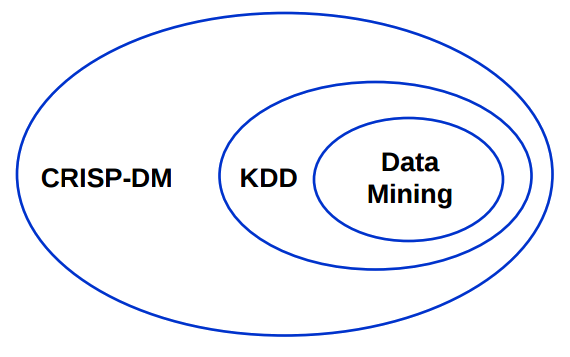
\includegraphics[width=100mm, height=60mm]{Figuras/BigData/RelacaoCrispKddDm.png}\\
\tiny Fonte: Neurotech -- 2012
\end{figure}

%\pagebreak

\subsection{Ciclo de vida do CRISP--DM}

O modelo de processo CRISP--DM provê seis fases para um projeto de mineração de dados, sendo assim determina-se um ciclo de vida 
compreendido para cada uma dessas fases:

A figura 2.2 ilustra as fases do ciclo:

\begin{figure}[!ht]
\centering
\caption{O padrão CRISP-DM \cite{Crisp2000}}
\vspace{1mm}
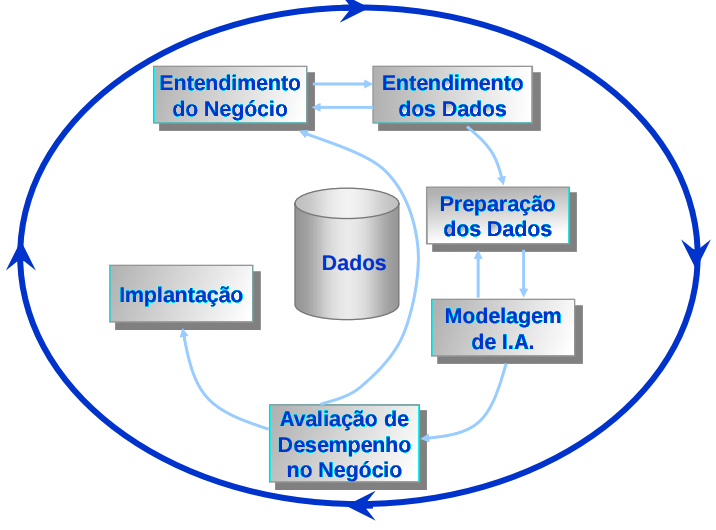
\includegraphics[width=120mm, height=90mm]{Figuras/BigData/CrispDM2.png}\\
\tiny Fonte: CRISP-DM 1.0
\end{figure}

\vspace{0.5cm}

A primeira fase, conhecida como \textbf{Entendimento do negócio}, ou ``fase de entendimento dos objetivos e dos requerimentos sob a 
perspectiva do negócio'' \cite{Crisp2000} é uma fase crucial da mineração,  um especialista (ou muitos) deve ser consultado. 
O analista de dados e o analista do negócio traçam os objetivos da mineração sob a perspectiva do cliente. Questionamentos incorretos 
ou negligência nesta fase podem acarretar esforços excessivos no processo como um todo a experiência de um profissional da área 
é condição ``sine qua non'' nessa fase. Portanto avaliar o negócio, avaliar a situação sob o ponto de vista dos riscos de não conclusão 
do processo, determinar os objetivos e traçar um plano para execução. Essas etapas são delineadas nas figuras que se seguem. A figura 2.3 é sobre o Entendimento do negócio já descrito anteriormente.

\vspace{0.5cm}

\begin{figure}[!ht]
\centering
\caption{Entendimento do negócio}
\vspace{1mm}
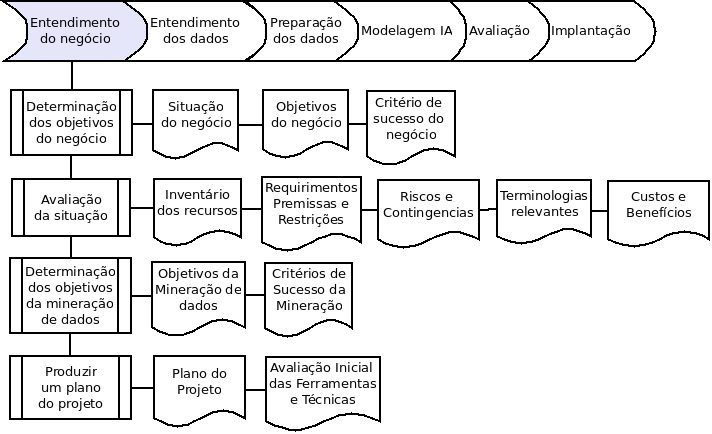
\includegraphics[width=160mm, height=120mm]{Figuras/Cronograma/Entendimento.png}\\
\tiny Fonte: CRISP-DM 1.0 (adapatado)
\end{figure}

\pagebreak

\vspace{1.5cm}

Em seguida, o analista de dados passa à segunda fase, \textbf{Entendimento dos dados}, na figura 2.4. Essa fase caracteriza-se pelo exame acurado dos dados, procurando identificar sua qualidade. 
Dados ausentes -- ``missing data'' -- são comuns em bases de dados não estruturadas, configurando-se como
um problema a ser considerado, pois seu tratamento pode consumir muito tempo do analista de dados, estima-se cerca de 80\% do tempo total \cite{DataMining}. 

\vspace{0.5cm}

\begin{figure}[!ht]
\centering
\caption{Entendimento dos dados}
\vspace{1mm}
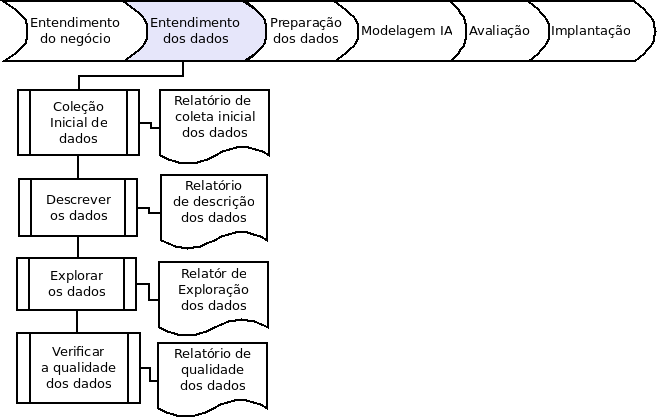
\includegraphics[width=160mm, height=120mm]{Figuras/Cronograma/EntendDados.png}\\
\tiny Fonte: CRISP-DM 1.0 (adapatado)
\end{figure}

%\vspace{0.5cm}
\pagebreak


A terceira fase, \textbf{Preparação dos dados}, figura 2.5, diz respeito à construção final do conjunto de dados. 
Preparar os dados significa, criar e selecionar atributos, criar tabelas ou planilhas e registros dos dados.
Para selecionar quais dados serão mais relevantes, calcula-se, por exemplo, o coeficiente de correlação linear entre os atributos (variáveis), quando as variáveis são numéricas. Outra forma de qualificar os dados é calculando a quantidade de informação que cada atributo possui. A máxima entropia de cada atributo pode fornecer informações sobre a qualidade da variável quando esta estabelece ganho de informação \cite{NorvigRussel2004}, vide equação da Entropia \footnote{O conceito de entropia será discutido na seção 2.6.2, referente a Árvores de Decisão}: $ H_{x}=-\sum_{\forall x \in X}P(x)log_{2}P(x) $
Onde $ H_{x} $ é a medida de entropia, x um atributo do conjunto de variáveis $X$ de variáveis. 

\vspace{0.5cm}

\begin{figure}[!ht]
\centering
\caption{Preparação dos dados}
\vspace{1mm}
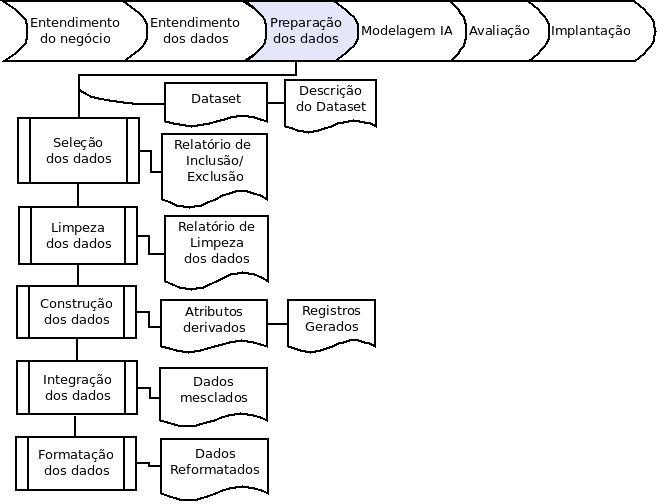
\includegraphics[width=160mm, height=120mm]{Figuras/Cronograma/PreparaDados.png}\\
\tiny Fonte: CRISP-DM 1.0 (adapatado)
\end{figure}

\pagebreak



Na quarta fase, \textbf{Modelagem de I.A.}, figura 2.6, a tecnologia deve ser escolhida de forma criteriosa, baseada também na experiência do analista de dados. 
Em sistemas de suporte à decisão, uma tecnologia inadequada pode levar a decisões imprecisas. É comum retornar às fases anteriores para adequar a técnica aos dados. 
Um modelo de regressão logística para problemas binários, redes neurais para problemas de classificação, e assim por diante.

\vspace{0.5cm}

\begin{figure}[!ht]
\centering
\caption{Modelagem IA}
\vspace{1mm}
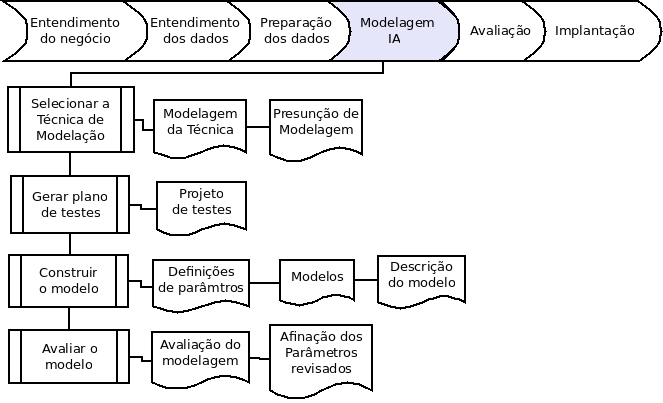
\includegraphics[width=160mm, height=120mm]{Figuras/Cronograma/Model_IA.png}\\
\tiny Fonte: CRISP-DM 1.0 (adapatado)
\end{figure}

%\vspace{0.5cm}
\pagebreak

Na fase cinco, \textbf{Avaliação de desempenho}, figura 2.7, um ou muitos modelos devem ter sido construídos e testados, 
de forma que seja possível atingir uma alta qualidade do ponto de vista da análise dos dados, ou seja, que o 
modelo proposto esteja de adequado aos objetivos do negócio. Para tal é preciso que antes do desenvolvimento final 
do modelo, os passos executados até então sejam avaliados e revistos.

\vspace{0.5cm}

\begin{figure}[!ht]
\centering
\caption{Avaliação do modelo}
\vspace{1mm}
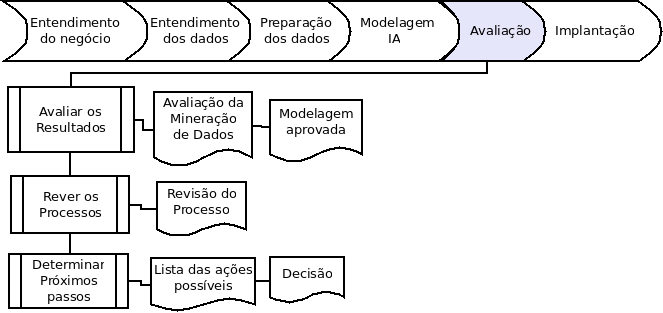
\includegraphics[width=160mm, height=120mm]{Figuras/Cronograma/Avaliacao.png}\\
\tiny Fonte: CRISP-DM 1.0 (adapatado)
\end{figure}

\pagebreak

A sexta e última fase caracteriza-se pela conclusão do modelo, figura 2.8. No entanto, a criação do modelo não é o fim do processo.
O conhecimento adquirido precisa ser incrementado, organizado e apresentado de maneira que o cliente possa usá-lo.
É importante ressaltar que este ciclo poderá ser retomado até que o modelo esteja adequado às necessidades e especifidades do cliente.

\vspace{0.5cm}

\begin{figure}[!ht]
\centering
\caption{Implantação do modelo}
\vspace{1mm}
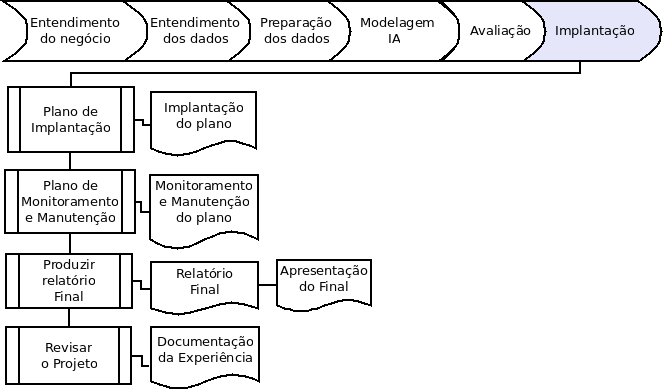
\includegraphics[width=160mm, height=120mm]{Figuras/Cronograma/Implantacao.png}\\
\tiny Fonte: CRISP-DM 1.0 (adapatado)
\end{figure}

%\section{Além do KDD -- \textit{Domain-Driven for Data Mining}}

\pagebreak

\section{Mineração de dados}

No processo de extração do conhecimento, também conhecido como \textit{Knowledge Discovery Databases} (KDD), um dos importantes passos a ser considerado é a mineração de dados, que se caracteriza pela aplicação de algoritmos 
específicos para descoberta de padrões e/ou comportamentos em grandes bases de dados, também conhecido como repositórios de dados \cite{FayyadUeoutros}.

A mineração se distingue das técnicas estatísticas pelo fato de que  não trabalha com dados hipotéticos, mas se apoia nos próprios dados para extrair os padrões \cite{Castanheira2008}. 

FAYYAD \cite{FayyadUeoutros}, destaca que é necessário distinguir claramente KDD e mineração de dados. Enquanto que a descoberta de conhecimento em bases de dados (KDD) é um processo dividido em etapas bem distintas (Figura 2.9), a Mineração de Dados (MD) é um passo no interior desse processo. 
Todavia, esse passo é de considerável relevância para que se possa extrair conhecimento adequadamente. 
A aplicação “cega” dos métodos de mineração de dados, ainda segundo Fayyad \cite{FayyadUeoutros}, pode conduzir à descoberta de dados sem significado e a padrões inválidos. 

Nos repositórios dos dados abertos do governo federal \cite{Dados-BR} existem vários tipos de dados e informações, nesses repositórios que podem ser minerados, contudo esses dados, inicialmente são selecionados e agrupados, a seguir passam por uma fase de preprocessamento, que consiste em tratá-los de forma a prepará-los para a mineração. Essa fase é de fundamental importância na estruturação dos dados, uma vez que em grandes volumes de dados, também conhecido ``Datawarehouse'' \footnote{Em Datawarehouse os dados também são estruturados, mas de uma maneira específica, que permitam aplicar técnicas conhecidas como Business Intelligence } \cite{RalphKimball2013}, podem existir inconsistências, faltas (missing data) ou 
duplicidade e erros de informações.

As técnicas de mineração de dados trabalham com dados estruturados, preenchidos em sua totalidade sem \textit{missing data}, para poder extrair informações relevantes.
Existem várias maneiras de se contornar os dados ausentes, como o preenchimento dos dados através de técnicas de inteligência artificial, da média dos valores; em dados numéricos 
ou com a moda; quando os dados forem categóricos \footnote{Dados categóricos são dados textuais que identificam uma categoria de dados}. Os dados são apresentados como uma tabela onde a primeira coluna ficam as variáveis (qualitativas ou quantitavis), em seguida vém os dados que seguem segundo a primeira linha a correspondência de que tipo eles são. 

Normalmente são criadas variáveis a partir dos dados numéricos para ampliar o conhecimento sobre esses dados. Para cada tipo de dado (numéricos, categóricos) existem técnicas apropriadas para serem aplicadas sobre eles, algumas mais sensíveis às problemáticas elencadas anteriormente
e outras mais robustas \cite{DataMining2}, que por sua vez estão associadas a classes de problemas que a mineração trata, a tabela 2.1 (página 19) delineou o domínio.

O caminho desde a coleta dos dados até sua mineração e extração de conhecimento é longo, a figura 2.9 tem a ilustração desse caminho:

\begin{figure}[!ht]
	\centering
	\caption{Fases da mineração de dados até extração do conhecimento}
	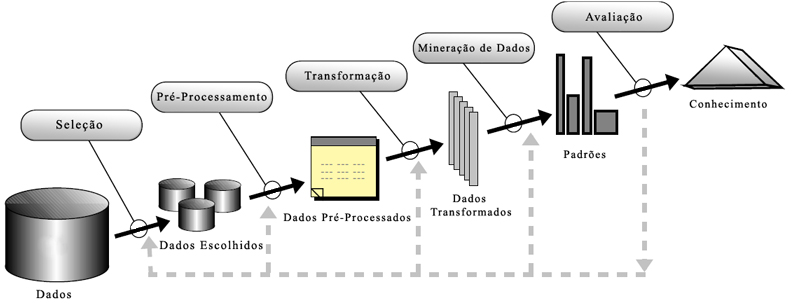
\includegraphics[width=140mm, height=60mm]{Figuras/BigData/Fayyad.png}
\end{figure}

\pagebreak


Na origem dos dados, os ``inputs'' estão representados na figura onde se lê ``Dados''. Estes geralmente estão repletos de \textit{missing data} e/ou dados inconsistentes, conhecidos como dados não estruturados. 
O balão onde se lê ``Seleção'' representa a coleta das informações ou a seleção dos dados em grandes repositórios de dados como Datawarehouse ou \textit{Big Data}. \footnote{A definição de Big data se encontra na página 16}.


Em nossa pesquisa esses dados são provenientes das mais diversas fontes, tais como, redes sociais, câmaras de trânsito, informações de satélites meteorológicos e outras fontes.

Armazenar dados provenientes de redes sociais nessa etapa pode ser um grande problema, devido à sua extensão, porém os dados relevantes podem ser armazenados em ``Dados Escolhidos'' 
com tecnologia apropriada, utilizando-se técnicas de ``Map'' e ``Reduce'' ou mineração de dados em textos \textit{Text Mining} para criar \textit{cluster} de informações e ler os fluxos de dados (stream data). 
Algumas técnicas de IA podem ser aplicadas nessa etapa como, ``Data Mininng Swarm Robotics'' através de Botnets \footnote{Botnet é citado no sentido da coleta de informações} ou ``Swarm Intelligence''.

No balão ``Pré-Processamento'' os dados não-estruturados são tratados, por exemplo, retirando os \textit{missing data}. 
Para estruturar as informações é preciso utilizar técnicas linguísticas, uma vez que existe lógica entre eles \cite{Aranha2006}.
Esses dados normalmente são coletados por técnicas de Mineração de Textos, também conhecidas como Mineração de Dados em Textos, técnicas de IA como ``Machine Learning'' 
têm sido muito utlizadas. Em ``Transformação'' os dados foram em estruturados, podendo ser armazenados em Bancos de Dados, conhecidos como Datawarehouse, por exemplo o Hive \cite{NoSQL2015}. \footnote{Hive é um de Datawarehouse que armazena dados não estruturados: \textit{Not Only SQL ou também Not structured SQL} NoSQL. Ferramentas NoSQL servem para trabalhar com o \textit{Big Data}, outros exemplos: HBase, MongoDB e Pig}.

O processo de Mineração dos dados começa no balão ``Mineração de Dados'', onde são aplicadas as técnicas de IA conhecidas como classificadores, para extração de padrões, tais como: 
``Decision Tree'' (Árvore de decisão), ``Artificial Neural Network'' (Redes neurais artificiais), ``Logistic Regression'' (Regressão Logística), ``Naïve Bayes'' e ``Deep Learning'', detre outros.
Algumas técnicas de mineração de dados são fortemente influenciadas pelas informações na entrada (input), como as Árvores de decisão \cite{DecisionTree}. 
As Redes Neurais, dependendo da quantidade de variáveis de entrada, paderão ter milhares de neurônios na camada intermediária, o que inviabilizaria essa metaheurística 
\footnote{Metaheurística são heurísticas aplicadas a problemas em que os custos computacionais não são tratáveis em tempo polionomial, devido às explosões combinatórias geradas
pelo grande número de tentativas. Metaheurísticas bioinspiradas metaforizam o comportamento de animais sociais, tais como formigas, pássaros, peixes e outros}.

Todas essas etapas descritas na figura 2.9 são recorrentes, como indicam as setas pontilhadas que retornam aos passos anteriores.
Utilizar técnicas de mineração de dados, extrair dados e conhecimentos, com isso pode-se predizer os resultados futuros na saída do modelo, 
quando determinados dados ocorrem na entrada \cite{Amin2015a}; essa técnica é o \textit{Knowledge Discovery Databases}.
O KDD utiliza métodos de Aprendizagem de Máquina para efetuar essa extração.


%\pagebreak


\section{Mineração em Dados Textuais} %\label{arte:palavraChave:DataMiningBigData}

A mineração em dodos textuais ou Mineração em Textos, tal como acontece com a mineração de dados vai buscar os dados em arquivos tipo textos digitalizados, contudo esses arquivos são transformados em documentos antes de serem analisados pelos algoritmos de IA.

De acordo com Hotho, Nürnberger e Paass  \cite{hotho2005brief} a expressão \textit{Text Mining} ou descoberta de conhecimento em textos foi referendada em 1995. Entretanto o interesse por extrair conhecimento oriundo de textos remonta à década de 60' \cite{stone1968general}. Hotho, Nürnberger e Paass  \cite{hotho2005brief} discutem, ainda, que é frequente a confusão de termos. Esses mesmos autores \cite{hotho2005brief} na tentativa de definir \textit{Text Mining} afirmam que é preciso considerar a perspectiva específica da área, definindo três possibilidades:

\begin{enumerate}
	\item A perspectiva sugere que \textit{Text Mining} corresponde à extração de fatos do texto, ou seja, extração de informação;
	\item A abordagem assume que mineração em texto se configura como a aplicação de algorítimos e métodos do campo de \textit{Machine Learning}, cujo objetivo seria encontrar padrões usuais;
	\item A perspectiva prevê que a mineração em textos segue o modelo de processo de descoberta de conhecimento. É frequente na literatura, a cerca da mineração em texto, entendê-la como uma séria de passos para extração de informação bem como o uso de mineração de dados ou processos estatísticos.
\end{enumerate}

Embora as pesquisas no campo da mineração em textos sejam relativamente recentes, os estudos envolvendo Processamento de Linguagem Natural (Natural Language Processing -- NLP) datam da década de 40' \cite{liddy2001natural}. 

As primeiras aplicações computacionais relacionadas à linguagem natural aparecem em torno de 1946 \cite{liddy2001natural},  decorrente da expertise de Alan Turing para quebra de códigos inimigos durante a segunda guerra mundial. 

Ainda segundo Liddy \cite{liddy2001natural} outro importante avanço é identificado no final da década de 50' quando Noam Chomsky introduziu a ideia de Gramática Gerativa. Neste mesmo período começaram a surgir pesquisas no campo do reconhecimento da fala. 

Desde então, essa área de conhecimento tem experimentado grandes avanços, particularmente, nos tempos atuais, com a Mineração em Textos nas Redes Sociais.

A Mineração em textos é inspirada em técnicas de \textit{Machine Learning} \cite{Aranha2006}. Todavia, analisar textos é basicamente entender o seu significado, baseado em regras de associação lógica. O mapa mental na Figura 2.10 mostra um modelo de análise de texto feito por seres humanos.

\begin{figure}[htpb]
	\centering
	\caption{Mapa mental da Mineração em textos}
	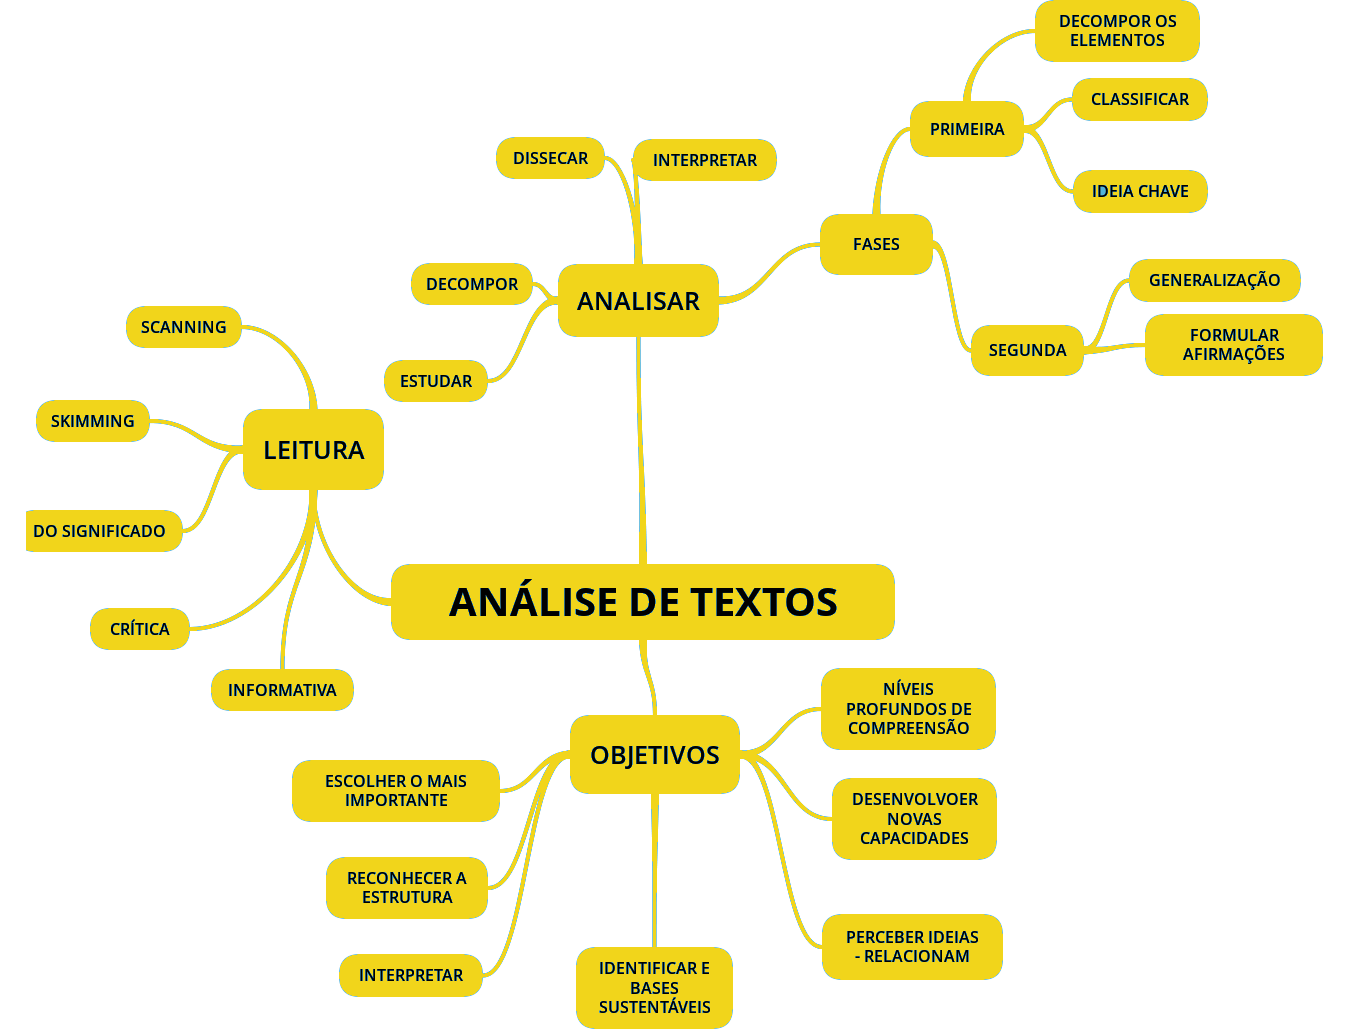
\includegraphics[width=160mm, height=90mm]{Figuras/BigData/Analise_Textos2.png}\\
	\tiny Fonte: o autor
\end{figure}


Minerar dados em texto é um processo que deve ser divido em várias etapas \cite{Lima2012}. Minerar em redes sociais exige ao menos mais uma etapa: a escolha de uma rede social, cada uma delas com sua tecnologia própria.

\subsection{Mineração em Textos nas Redes sociais}

%\subsubsection{Introdução ao estudo das Redes Sociais}

As redes sociais têm assumido, nos dias atuais, um papel essencial na vida de seus usuários. Não apenas como espaço de descontração, mas, sobretudo, como lugar de troca de informações que permitam, dentre outras coisas, tomar conhecimento acerca dos acontecimentos, sejam eles locais ou globais, que influenciarão sua vida. De modo particular, nos grandes centros urbanos, as redes sociais têm servido de fonte de conhecimento acerca de segurança pública, mobilidade urbana e acontecimentos de toda sorte, que possam fazer com que, por exemplo, uma pessoa resolva seguir um ou outro caminho para chegar a um determinado lugar, quer seja ele próximo ou distante de onde se encontre \cite{sarker2015utilizing} \cite{madden2013teens} \cite{naaman2010really}.

Além da troca de informações momentâneas, as redes sociais permitem uma atualização praticamente em tempo real, a partir da utilização de seus usuários e de instituições que também dela fazem uso (por exemplo, a Polícia Rodoviária Federal), de modo que possibilita que decisões sejam tomadas e reorientadas, em virtude da alimentação das informações nas redes.

No que diz respeito às escolhas relacionadas ao trânsito, sejam relativas as áreas urbanas, bem como a centenas de quilômetros adiante, pelo interior de um estado, cada vez mais as pessoas não tomam decisão sem antes consultar aplicativos e redes sociais tais como o waze, twitter, facebook, etc.

Aplicativos para celulres até dispõem de GPS, Google Maps e outras fontes que lhe orientem sobre melhores rotas, que levem com maior rapidez e segurança ao seu destino.

Se pensarmos no transporte de cargas, a principal função das redes sociais não é de caráter lúdico, mas, sim, como uma ferramenta essencial para que não haja qualquer contratempo que possa causar prejuízo à empresa ou empresas envolvidas. 
Afinal de contas, no que tange ao transporte de mercadorias, sempre há pelo menos duas empresa relacionadas: a de produção do bem e a de transporte do mesmo ao seu destino.

O que discutimos até agora é amplamente sabido por aqueles que analisam o uso das redes sociais na atualidade. O que pretendemos, então, é trazer uma contribuição de natureza científica a essa compreensão e à utilização de forma cada vez mais eficaz dessas ferramentas, a partir do uso da IA, da mineração de dados e dos métodos de extração e produção de conhecimentos (KDD).


O crescimento dos dados eletrônicos, nos últimos anos, até 2020, pode ser acompanhado na tabela 2.2. Esta demonstra o volume de dados e informações produzidas no mundo entre 2000 à 2020. "Em 2010 empresas e usuários armazenaram mais de 13 exabytes de novos dados" \cite{bigdataQualquerUm}.

%tabela 5
\begin{table}[!ht]
	\centering
	\caption{Volume de dados no mundo}
	\vspace{1mm}
	\begin{tabular}{l|c|c|c}
		\hline
		\textbf{Ano} & \textbf{Qtd} & \textbf{Unidade} & \textbf{Múltiplo}\\
		\hline
		2000 & 800 & terabytes – TB & $10^{12}$\\
		2006 & 160 & petabytes – PB & $10^{15}$\\
		2009 & 500 & exabytes – EB & $10^{18}$ \\
		2012 & 2,7 & zettabytes – ZB & $10^{21}$\\
		2020 & 35 & yottabytes – YB & $10^{24}$\\
	\end{tabular}
\end{table}

Uma parte desses dados são as redes sociais. A rede social escolhida para esta pesquisa foi o Twitter por apresentar características como API aberta de fácil conexão para obtenção dos dados. Uma rede social é sobretudo uma de conexão entre pessoas, contudo, sob o ponto de vista tecnológico uma conexão entre nós e arestas, os nós simbolizam as pessoas e as arestas a ligação entre elas, essa ``arquitetura social'' é conhecido como grafo. A figura a 2.11 foi gerada pelo software Gephi \cite{ICWSM09154} representa um grafo da rede social Twitter.

\begin{figure}[!ht]
	\centering
	\caption{Grafo de uma rede do Twitter}
	\vspace{1mm}
	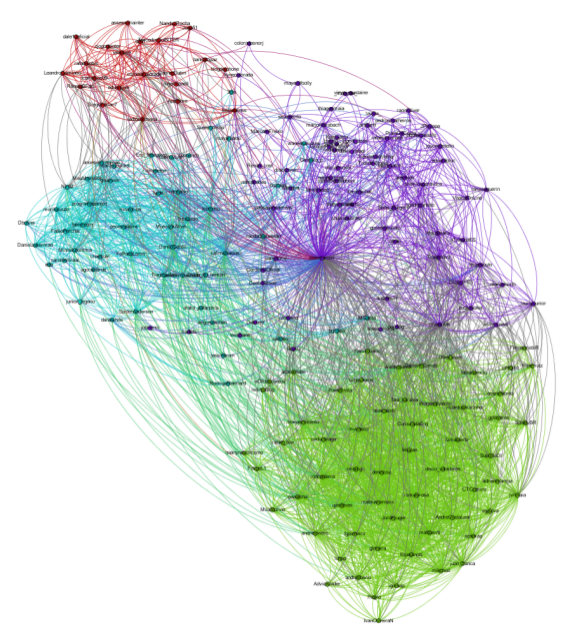
\includegraphics[width=120mm, height=65mm]{Figuras/BigData/grafoExemplo.png}\\
	\tiny Fonte: https://github.com/gephi/gephi/wiki/Official-papers. Acessado em: 10/03/2017
\end{figure}


%\pagebreak

\subsubsection{O Twitter}

O Twitter caracteriza-se como um microblog onde os usuários escrevem em um espaço delimitado (cerca de 140 caracteres) sobre os mais diversos assuntos. Tais usuários conectam o aplicativo por meio de uma multiplicidade de dispositivos: computadores, tablets e celulares, formando uma grande rede social mundial. Essa rede possui duas diferentes APIs, responsáveis pela captura dos dados: Rest API e Streaming API. O Twitter funciona com o padrão de arquivos JSON e os dados são capturados nesse formato \cite{francca14big}. A cada dia centenas de terabytes são inseridos nos seus bancos de dados, conhecidos como Hadoop data warehouse, tornado impossível capturar todas as informações produzidas em um largo espaço de tempo, portanto ou se analisa o Streaming de dados ou a API.

A ideia inicial do Twitter, segundo seus fundadores, era de que essa rede se comportasse como um “SMS da Internet” (30). As informações são enviadas aos usuários, conhecidas como twittes, em tempo real e também enviadas aos usuários seguidores que tenham assinatura para recebê-las: os seguidores. A conexão entre os usuários da rede social se deve à relação entre os seguidores e os seguidos. O comportamento do seguidor para retweetar os usuários seguidos serve como principal mecanismo para compartilhar informações nessas redes.

Nas pesquisas que envolvem as redes sociais, analisar o conteúdo utilizando ferramentas de mineração de textos é um procedimento frequente e tem apontado resultados surpreendentes sobre o comportamento social e suporte à tomada de decisão \cite{abrahams2015integrated}. É comum, ainda, aplicar mineração de textos em bibliotecas e outras instituições. Isso implica em rastrear tópicos, extrair informações, agrupar, categorizar \cite{fan2006tapping}.

Em recente artigo, Sandhu \cite{sandhu2015scheduling} indicou a importância do aprendizado sobre mineração de dados e ferramentas de Big Data para as bibliotecas acadêmicas, de forma a melhorar a eficiência da biblioteca e dos serviços de informação. Similarmente, Zhang e Gu \cite{zhang2011text} alegaram que minerar conhecimento sobre os clientes é importante para as bibliotecas acadêmicas. Na mesma linha de investigação, Sarker et al. \cite{sarker2015utilizing} destacam que a abordagem da mineração de textos para os dados das mídias sociais tem sido utilizada em muitos campos, como negócios, ciência da saúde, dentre outros. 

Estudos atuais têm mostrado o papel da análise sentimental e mineração de opinião nas redes sociais, em particular no Twitter, como forma de investigar padrões de comportamento \cite{pak2010twitter} \cite{kumar2012sentiment}.

%(FONTE: Artigo “Library \& Information Science Research)

Outro estudo aponta que em 2013 um número superior a 70\% dos indivíduos adultos que faziam uso da internet estavam conectados a redes sociais. Cerca de 20\% utilizavam o twitter, sendo que aproximadamente 46\% conectando-o diariamente e algo em torno de 29\% mais de uma vez ao dia \cite{madden2013teens}. 

Um relatório publicado em 2013 revelou que o Twitter estava posicionado entre as três maiores mídias sociais, em termos de adesão e utilização, perdendo apenas para o facebook e o youtube. Esse relatório revelou, ainda, que naquele ano, nos EUA 8\% dos adultos que tinham entre 18 e 29 anos de idade utilizavam o twitter como principal mídia social. Em outras idades, esse percentual subia para 45\% no mesmo país. As notícias são o principal interesse dos usuários dessa rede \cite{mitchell2013news}. 

Em 2014, os dados revelavam que, em um dia típico, sem qualquer evento extraordinário, essa rede era conectada por cerca de 230 milhões de usuários, responsáveis pela produção de aproximadamente 500 milhões de ``tweets'' (postagem tipo microblog) (Twitter, 2014).

Naaman, Boase e Lai \cite{naaman2010really}, classificaram os   conteúdos propagados nos tweets em oito categorias: Informações compartilhadas, auto promoção, opinião/queixas, declarações e pensamentos aleatórios, ``eu agora'' (me now), perguntas aos seguidores, manutenção de presença e piadas. 

Na Web, por sua vez, a quantidade de citações (i.e. links de URL) e estrutura dos links são utilizadas pelos motores de busca (ex: o Google) com o objetivo de identificar a relevância e aceitação de \textit{websites} \cite{brin1998anatomy}, em decorrência do número de seguidores, da quantidade de menções feitas, de ``retweets'', por exemplo.

Cha, Haddadi e Benevenuto \cite{cha2010measuring} avaliaram a influência dos usuários no Twitter na rede, como um todo, analisando o número de ``retweets'', menções e seguidores. Esses pesquisadores identificaram uma correlação positiva entre o número de seguidores e o número de ``retweets'' pelo top 10 (do Twitter) e o primeiro percentil dos mais conectados, com base no grau do link (i.e. número de seguidores). 


\subsubsection{Modalidades e ferramentas de análise do Twitter} 

Nesse tópico abordaremos, em maior detalhe, as escolhas metodológicas e ferramentas analíticas utilizadas em estudos que levam em conta dados do twitter, apresentando alguns dessas pesquisas.

Em artigo conduzido por Chu \& Du \cite{Chu2012}, os autores justificaram que as mídias sociais têm sido utilizadas cada vez mais para promoção das bibliotecas, com o objetivo de incrementar a relação com os clientes, permitindo “facilitar informações e compartilhar conhecimentos, incrementar serviços e promoções, interação com estudantes usuários das bibliotecas, a um custo mínimo” (p. 72) (livre tradução do autor) \footnote{Facilitate information and knowledge sharing, service enhancement and promotion, interaction with student library users, at minimal costs.}. Tal prática têm promovido considerável mudança na interação com usuários e relacionamento com os clientes \cite{del2012libraries}, tendo sido utilizada frequentemente como alternativa para estabelecer uma conexão personalizada com os seus usuários \cite{boateng2014web}. 

A pesquisa em questão interessou-se em investigar quantas vezes a biblioteca acadêmica usa o Twitter; tipo de conteúdo compartilhado pela biblioteca acadêmica no twitter; temas associados com os ``tweets'' da biblioteca acadêmica \cite{Al-Daihani2016}. Nesta pesquisa foi obtido a partir da ``timeline'' de dez bibliotecas acadêmicas (i.e. todos ``tweets'' desde a adesão à plataforma), através de um serviço de arquivamento (twimemachine.com), em dezembro de 2014. Foram selecionadas as 10 maiores bibliotecas ranqueadas pelo Shanghai Ranking, tendo a seleção se restringido às universidades de língua inglesa e a apenas uma biblioteca por instituição, para o caso de a universidade ter mais de uma. 

Na etapa de preprocessamento -- ``dataset preprocessing'' -- o grupo de dados recuperado foi tratado, para reduzir os ``ruídos'', seguindo uma abordagem consistente com outros estudos de mineração em textos, tal como o de Ralston, O'Neil, Wigmore e Harrison \cite{ralston2014exploration} e de Yoon, Elhadad e Bakken \cite{yoon2013practical}. O processo contemplou a aplicação de certo número de filtros. Por exemplo, foram removidas as ``stopwords'', pontuação e numeração, todos os nomes de usuários seguido por um símbolo ``\@'', ``hashtags'' após o símbolo ``\#'' e ``hyperlinks'' após o ``http''. Também foi removido a abreviação do Twitter tal como ``RT'' (retweetes), e ``MT'' (tweet modificado) e palavras tal como ``via''. O nome do usuário do Twitter para cada biblioteca acadêmica também foi excluído. 

Para análise do conjunto de dados, utilizou-se a mineração em textos e para investigar os históricos de ``tweets'' das bibliotecas escolheu-se a análise de conteúdo. A frequência dos ``tweets'', ``retweets'' e sua distribuição foi identificada e contabilizada. Em seguida, os ``tweets'' marcados com o PamTaT \footnote{ Ferramenta ``text mining'' desenvolvida por Pamplin Collage do Instituto Politécnico de Negócios de Virgínia da Universidade Estadual de Virgínia (Bird, Loper \& Klien, 2009)}. 

Quando se tem um \textit{corpus linguístico} ou, em outras palavras, um documento que está sendo analisado, baseado nas informações linguísticas que ele contém, uma ferramenta estatística frequentemente utilizada em mineração de textos é a TF-IDF. Esta sigla é a abreviação, em língua inglesa, de \textit{Term Frequency}, isto é, \textit{frequência do termo}, e \textit{Inverse Document Frequence} \cite{hiemstra2000probabilistic}, que significa frequência inversa do documento. Em termos gerais, o TF considera que o peso de uma palavra em um documento está relacionado à frequência com que essa palavra aparece no mesmo. Em nossa pesquisa, a palavra ``acidente'', quando temos o trigrama \textit{ocorrência de acidente}, as palavras \textit{ocorrência} e \textit{acidente} têm um importante peso relacionado a frequência, enquanto que o \textit{de}, sem estar acompanhado dos outros dois, não tem significado relevante para os dados minerados, pois o mesmo deverá aparecer inúmeras vezes, sem estar relacionado ao que é investigado. Nesse caso, o IDF aponta exatamente para a \textit{frequência inversa}, ou seja a palavra \textit{acidente} é provável que apareça no texto em menor frequência que \textit{ocorrência}, portanto a ordem inversa  deverá ser: ``acidente'' < ``ocorrência'' < ``de'', como pretendíamos. 
A equação 2.1 demonstra como se encontra o \textit{idf}.
\begin{equation}
idf(term) = \ln(\frac{n_{documents}}{n_{documents\  containing \ term}})
\end{equation}

 A técnica serve, para determinar a frequência de palavras simples (unigrams), de duas palavras (bigrams) e sequência de três palavras (trigrams) que aparecem no texto fonte. Com isso, permite desenvolver uma matriz de frequência de termos-tweet, mostrando como sequências de palavras simples e múltiplas palavras (n-grams) são usadas pela biblioteca acadêmica selecionada. 



\begin{figure}[htbp!]
	\centering
	\caption{Descrição da conta Twitter das bibliotecas acadêmicas}
	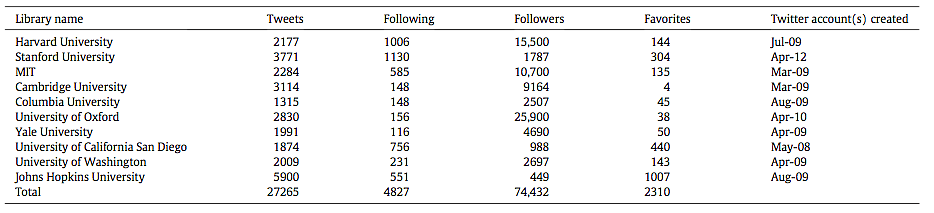
\includegraphics[width=175mm, height=70mm]{Figuras/Twitter/contaTwitter.png}\\
	\tiny Fonte: AL-DAIHANI, S. M. and ABRAHAMS, A. -- 2016
\end{figure}

Observa-se que foi incluído o número de ``tweets''; a quantidade de usuários seguidos pela biblioteca; a quantidade de seguidores e o número de ``tweets'' favoritos da biblioteca. A Universidade Johns Hopkins, como se pode observer na tabela, tem o maior número de
``tweets'', seguida pela biblioteca da Stanford University e pela biblioteca da Cambrige University, respectivamente. A biblioteca da Universidade da Califórnia San Diego tem a conta do Twitter mais antiga (maio de 2008), mas apresenta um pequeno número de ``tweets'',
comparativamente à biblioteca da Stanford University, que começou no Twitter com uma conta em abril de 2012, mas possui o segundo maior número de ``tweets''. 


\begin{figure}
\centering
\caption{Bibliotecas de Universidades e contas no Twitter}
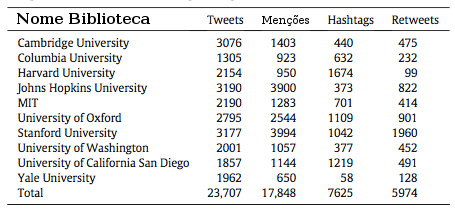
\includegraphics[width=0.7\linewidth]{Figuras/Twitter/contaPalavras}
\label{fig:contaPalavras}
\end{figure}

%\pagebreak

A análise do conteúdo dos Tweets foi desenvolvida da seguinte maneira: tomando a frequência de unigramas (palavras únicas), observou-se que a palavra mais frequente foi “open”, utilizada em uma variedade de contextos pelos ``tweets'' da biblioteca. Por exemplo: foi usada em um anúncio sobre a mudança do horário de funcionamento, bem como em um anúncio para abertura do espaço para os estudantes, exposições, abertura da casa (biblioteca), etc. 

\begin{figure}[ht]
	\centering
	\caption{Frequência de palavras}
	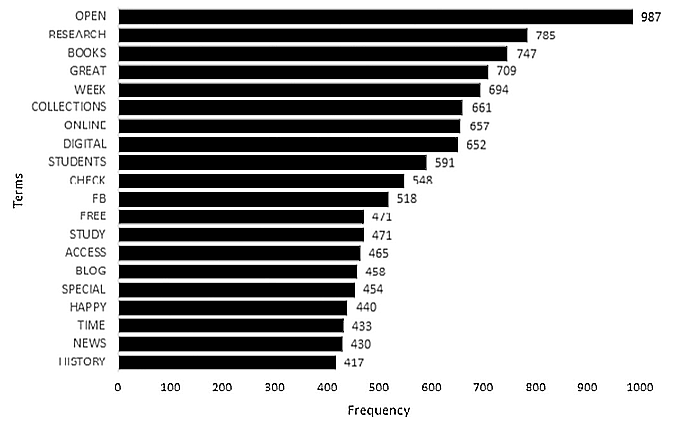
\includegraphics[width=0.6\linewidth]{Figuras/Twitter/ferqPalavras}\\
	\tiny Fonte: AL-DAIHANI, S. M. and ABRAHAMS, A. -- 2016
	\label{fig:ferqPalavras}
\end{figure}


O segundo termo mais frequente foi ``research'', que foi utilizado também em diferentes contextos, relacionados frequentemente a apoio, a investigação, por exemplo: workshop research, ferramentas de pesquisa e software, abertura ao acesso para pesquisar, dados e laboratório de pesquisas, guia de pesquisa e ajuda e campos de pesquisa. Outros termos tais como “livros”, “coleções” (acervos) e “on-line” foram utilizados no contexto dos ``tweets'' sobre os recursos da biblioteca. Tais termos foram incluídos em ``tweets'' relacionados a “e-books”, “textbooks”, “livros raros”, “solicitando e renovando livros”, “comentários de livros”, “novos livros”, “livros de coleções especiais”, “livros recomendados”, “política de circulação de livros”.

Na distribuição dos bigramas (sequência de duas palavras) no conjunto de ``tweets'', observa-se que o mais frequente foi “special collections”.
O segundo mais popular bigrama foi “open access”, utilizado em diferentes contextos, tal como política de acesso, publicidade, recursos, trenamentos e workshops, dicas e orientação, serviços, eventos e notícias. O resultado mostrou a ênfase colocada na iniciativa de promover “open access” com as instituições acadêmicas.

O terceiro maior bigrama foi “reading room”, relativo à atividade de suporte aos estudantes com as instituições acadêmicas. Essas salas são um dos mais importantes espaços da biblioteca, usadas para leitura e estudo. Os ``tweets'' eram, em sua maioria, relacionados a noticias de abertura e fechamento das salas de leitura: “reading rooms”.

Dentre os mais importantes trigramas (sequência de três palavras), destacou-se o trigrama “save the date”. Essa expressão era utilizada para requerer especial atenção dos seguidores para os eventos importantes que estavam para acontecer. Este trigrama é seguido, como o segundo mais frequente, por “pleased to announce”, outra expressão usada para enfatizar a importância de eventos especiais. O terceiro mais usado foi “open access week” (seguido muito próximo por “open access policy”), que novamente destaca os esforços na iniciativa de espaço aberto (open access). 

No caso particular da pesquisa em lide, o interesse voltou-se para os ``tweets'' da Polícia Rodoviária Federal do estado de Pernambuco, bem como de seus seguidores e de usuários que fizeram menção a eventos que afetam diretamente o tráfego nas principais rodovias do estado. A seguir, a título de exemplo, pode-se verificar uma sequência de ``tweets'' da Polícia Rodoviária Federal do estado de Santa Catarina:

\begin{figure}[htbp!]
	\subfigure{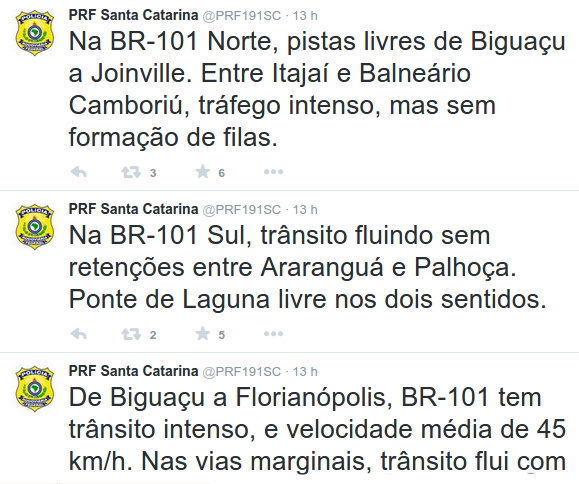
\includegraphics[width=60mm, height=48mm]{Figuras/BigData/twittePRF.png}}
	\quad \quad \quad \quad
	\subfigure{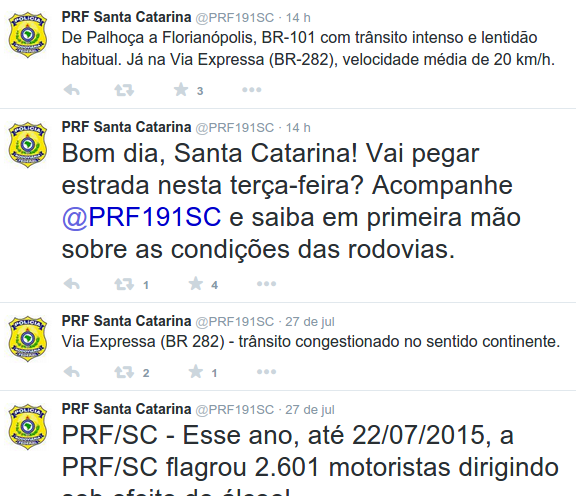
\includegraphics[width=60mm, height=48mm]{Figuras/BigData/twittePRF2.png}}\\
	\centering \tiny Fonte: https://twitter.com/PRF191SC Acessado em: 10/10/2016
\end{figure}

A Polícia Rodoviária Federal disponibilizou às 13h através do canal @PRF191SC, informações relevantes sobre o trânsito naquela localidade, 
num espaço temporal variado. Por exemplo: entre Itajaí e Balneário Camboriú foi informado que o trânsito estava intenso, sugerindo que a frota de caminhões deva ter uma rota alternativa, caso a situação persista por muito tempo. No primeiro twitte da segunda coluna, é informado em Via Expressa (BR 282) que o trânsito está lento com velocidade de 20km/h (praticamente congestionado). 


Outra rede social conhecida pelos condutores de veículos é o Waze. O Waze é um aplicativo de navegação para o trânsito, e funciona em aparelhos celulares e tablets. Os utilizadores desse aplicativo são conhecidos como wazers e compartilham informações sobre o trânsito, em tempo real. Todavia, as informações somente estão disponíveis no momento em que são postadas pelos utilizadores, por um período de tempo pequeno. Caso não haja usuários trafegando pelas vias, ou caso os mesmos não tenham disponibilidade para compartilhar informações, não há o que se ver. Outro problema identificado em relação ao waze é que caso não haja conexão à Internet, não há como acessar os dados dos 'wazers', para navegação.

Além dos dados que chegam ao \textit{Big Data} através das redes sociais, as grandes cidades têm disponíveis câmeras de monitoramento do trânsito nos semáforos ou próximas a eles. Algumas com cobertura por canais de televisão, bem como câmaras de segurança próximas às rodovias, coletando informações em tempo real. Os dados desses dispositivos são gravados, sendo conhecidos como \textit{stream} de dados. Esses \textit{streams} podem ser disponibilizados na Internet, em sítios eletrônicos especialmente construídos para isso, como o http://vejoaovivo.com.br (acessado em 10/10/2016) dentre outros.

Os dados disponibilizados pelos diversos meios de comunicação não estão em formato que possam ser utilizados imediatamente, precisando antes serem processados. Tais dados não processados são conhecidos como ``dados frios''. O processo de tratar as informações, retirando-lhes o ``lixo'' e transformando dados ``frios'' em dados ``quentes'', é um processo que tem um custo temporal elevado, devido ao volume dos dados.


\section{Aprendizagem de Máquina} \label{arte:palavraChave:Machine}

Historicamente, a aprendizagem computacional está relacionada com ``o que'' há para ser aprendido \cite{Nilsson2005}. 
Para escolher o que aprender é necessário definir de ``onde'' ou sobre quais dados aprender.
Deve ser fornecido um conjunto de treinamento, para, em seguida, testar o conhecimento aprendido em um ``conjunto de teste''.

Aprendizagem de Máquina ou ``Machine Learning'' são métodos para analisar dados de forma automatizada e interativa.
Segundo Shalev-Shwartz \& Ben-David \cite{Ben-David2014}, o termo Aprendizagem de Máquina refere-se à detecção automatizada de Padrões de dados.

Para Nilsson \cite{Nilsson2005}, o aprendizado ocorre quando uma máquina modifica sua estrutura interna, programa ou dados 
(baseados nos inputs ou em uma resposta para informação externa) de tal maneira que melhora o desempenho futuro. Por exemplo, quando uma máquina de reconhecimento da fala melhora após ``ouvir'' várias amostras de fala humanas e que nós percebemos que está pronta, neste caso podemos dizer que a máquina aprendeu.

Sistemas que executam tarefas de inteligência artificial, tais como Reconhecimento de Padrões, Diagnóstico, Controle de Robôs, Predição e outros, precisam ser modificados para executarem ``Machine Learning'' \cite{Nilsson2005}.


\subsection{Tipos de Aprendizagem}

Quando se fala em algoritmos de IA, adentramos no campo de Aprendizagens e Máquinas. É o princípio da aprensizagem que faz com que o algoritmo estabeleça a decisão adequada para o problema proposto.
No campo da aprendizagem de máquina, é possível apontar três tipos de aprendizagem: a aprendizagem supervisionada, aprendizagem não-supervisionada e aprendizagem por reforço \cite{NorvigRussel2004}. As duas primeiras serão aqui descritas de maneira sucinta, e consideradas mais adiante, uma vez que interessam particularmente a essa pesquisa, sobretudo quando da utilização de redes neurais e árvores de decisão. 

A aprendizagem supervisionada \cite{Monard} se caracteriza pelo acesso ao conjunto de exemplos de treinamento pelo algoritmo de aprendizagem, também conhecido como indutor, de modo que haja especificação da saída desejada.
No caso da aprendizagem não-supervisionada \cite{NorvigRussel2004}, os valores de entrada são estabelecidos, mas não são definidos os valores de saída. O indutor terá o papel de estabelecer aproximações, propondo agrupamentos (clusters) em função de determinadas categorias como, por exemplo, similaridade \cite{Monard}.

Para ``aprender'' sobre uma determinada função \textit{f} definimos uma amostra em um conjunto de treinamento $X = {x_{1}, x_{2}, ...x_{n}}$.

As técnicas algorítmicas apresentadas nas seções subsequentes são parte da grande família de algorítimos que compõem 
o aprendizado de máquina aplicado a mineração de dados.

A descoberta de conhecimento através da aplicação das técnicas de mineração de dados podem ser agrupadas de acordo com suas funcionalidades \cite{DataMining2}, 
essas funcionalidades têm como característica principal a maneira como são descobertos os padrões no dados, elas podem estar 
em uma das duas categorias: tarefas descritivas ou tarefas preditivas. As tarefas mineração descritivas preocupam-se nas características 
dos dados no conjunto de dados; o ``data set''. As tarefas de mineração preditivas induzem regras nos dados correntes para produzirem 
predições \cite{DataMining2}. A seção seguinte analisa as tarefas preditivas.



\subsection{Algoritmos de Aprendizagem de Máquina}

\vspace{5mm}

Os algoritmos de Aprendizagem de Máquina selecionados para esta pesquisa contemplaram robutez, devido a grande quantidade de dados (cerca de 55 000 registros) a qualidade no tratamentos desses dados como e tolerância a falhas.
%\textbf{Introdução}


%
\subsubsection{Naïve Bayes}
\vspace{5mm}


Dentre os algoritmos de machine learning que destamos nessa dissertação está o Naïve Bayes. 
Essa classe de algoritmos é baseado no teorema da probabilidade condicional de Bayes \cite{montgomery2000estatistica}, que serve 
para rotular classes de variáveis independentes. O classificador Naïve Bayes é um modelo probabilístico relativamente simples, todavia, muito potente. Produz estimativas de probabilidade, em vez predições.


Um classificador Naïve Bayes produz probabilidade como output \cite{policarpo2015semantic}. A probabilidade que é produzida pode ser utilizada para distinguir a que grupo classificado, uma amostra não classificada pertence, por exemplo, dependendo da da mais alta probabilidade obtida entre um grupo de probabilidades.

Resumidamente, um classificador Naïve Bayes sugere que a presença ou ausência de um atributo particular de uma determinada classe não está relacionado à presença ou ausência de qualquer outro atributo. Ainda que esses atributos dependam entre si, ou da existência de outro atributo, esse tipo de classificador considera todas as propriedades como contributos independentes da probabilidade final \cite{policarpo2015semantic}.

Em mineração de dados variáveis independentes explicam a variável dependente para fazer predição.
Este classificador tem sido muito empregado para classificar documentos e detectar spam em mensagens. 
A probabilidade condicional pode ser explicada por um vetor $x = (x_{1}, x{2}, ..., x{n})$ que se representa \textit{n} características (variáveis independentes) que se atribui a estas instâncias de probabilidades $p(C_{k}|x_{i},...,x_[n])$ para cada \textit{K} possível ter vindo da classe $C_[k]$. Aplicando o teorema de Bayes da probabilidade condicional temos:

\begin{equation}
p(C_{k}|x) = \frac{p(_{k})p(x|C_{k})}{p(x)}
\end{equation}

Em outras palavras, a medida que se conhece os resultados das probabilidades pode-se predizer os novos resultados porque o conjunto de testes torna-se menor. A probabilidade condicional também pode ser entendida como:

\begin{equation}
p(posteriori) = \frac{p(priori) * verossimilhança}{evidencia}
\end{equation}

\vspace{5mm}

\textbf{Aprendizagem Bayesiana}
\vspace{5mm}

Baseado no teorema de Bayes, dado um conjunto de variáveis aleatórias $\omega = {x_{1}, x_{2},..,x_{n}}$ a variável aleatória \textit{H} (hipótese) denota o tipo de $\omega$, com valores possíveis para $h_{1}, h{2},...,h_{n}$. A medida que são inspecionadas as variáveis, são revelados os dados $D_{1}, D_{2},...,D_{n}$, onde $D_{i}$ é uma variável aleatória com valores possíveis para cada variável do conjunto $\omega$ de variáveis. Sendo D a representação dos dados do espaço de variáveis para uma predição sobre a parte desconhecida de \textit{X}, temos:

\begin{equation}
P(h_{i}|d) = \sum_{i}P(X|d,h_{i})P(h_{i}|d) = \sum_{i}P(X|h_{i})P(h_{i}|d)
\end{equation}
 onde cada hipótese $h_{i}$ determina uma distribuição de probabilidades sobre a variável \textit{X} \cite{NorvigRussel2004}.

Um aspecto relevante e positivo que deve ser mencionado acerca do classificador Naïve Bayes é que este requer apenas um pequeno grupo de dados de treinamento para estimar os parâmetros que são necessários para que seja feita a classificação. Outro aspecto que merece destaque é que ele se mostra eficiente para aprendizagem supervisionada, trabalhando de forma rápida com dados complexos \cite{policarpo2015semantic}.


\subsubsection{Árvores de Decisão}

%\textbf{Introdução}
\vspace{5mm}

No âmbito da inteligência artificial, quando se trata de algoritmos de aprendizagem, uma classe de algoritmos que tem se revelado potente para problemas das mais diversas naturezas é a árvore de decisão. Além do universo das pesquisas no campo da informática engenharia e ciências da computação, as árvores de decisão têm sido utilizadas, sobremaneira, em pesquisas relacionadas à Medicina, à Economia, nos mais diversos sistemas de suporte à decisão, como diagnósticos de doenças, investigação de fraudes, dentre outros \cite{Camilo}.

A escolha desse algoritmo está relacionada, em larga medida, a uma relação que cotidianamente chamamos de “custo benefício”. Uma árvore de decisão é gerada de maneira relativamente simples e os resultados produzidos são, em sua maioria - e a depender da área específica – de grande poder de abrangência e de fácil interpretação. Todavia, para que se faça opção por essa ferramenta, o pesquisador precisa ter clareza sobre a que classe de problemas ela atende, bem como, de que maneira pode ser gerada e realimentada, e de que forma seus resultados devem ser adequadamente interpretados.

Na pesquisa apresentada nessa dissertação, particularmente, as árvores de decisão possibilitaram grandes avanços na proposição do modelo de predição, conforme pode ser observado no capítulo dedicado aos resultados. 

Conforme o nome sugere, o que se espera de uma árvore de decisão é que ao final do processo resulte a melhor decisão. Todavia, para que a decisão satisfatória apareça, é necessário que o pesquisador faça as escolhas adequadas, de modo a poder tirar o melhor proveito dessa ferramenta. Para tal, é preciso compreender a natureza desse algoritmo e os processos a ele relacionados. A seguir serão apresentados os principais elementos que precisam ser conhecidos pelo pesquisador que deseja se aventurar por esse campo.

\vspace{5mm}
\textbf{Breve histórico e conceituação}
\vspace{5mm}

De maneira sintética, uma árvore de decisão tem como entrada um conjunto de atributos e como saída uma decisão. Os atributos podem, ainda, ser classificados de duas maneiras: discretos ou contínuos. Em virtude dos atributos de entrada, tem-se, como resultado uma função de valores discretos – aprendizagem de classificação – ou de valores contínuos – aprendizagem de regressão \cite{NorvigRussel2004}.

A decisão gerada aparece em função de uma sequência de testes executados, estando cada um deles relacionados a um nó da árvore. As ramificações que decorrem dos testes são o resultado encontrado a partir da realização do experimento. 
O exemplo a seguir ilustra uma árvore de decisão simples, onde se vê seu nó-raiz e suas ramificações. 


\begin{figure}[!ht]
	\centering
	\caption{Árvore de decisão}
	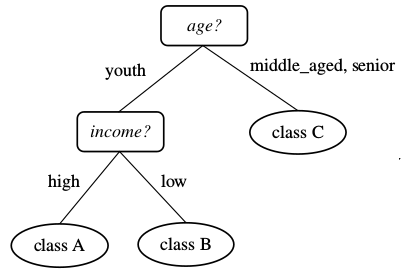
\includegraphics[width=60mm, height=45mm]{Figuras/Arvore/arvorejovem.png}\\
	\tiny Fonte: Han, J. and Kamber, M. 
\end{figure} 


Uma árvore de decisão obedece à regra básica “se-então”, de maneira que, parte-se do nó (se) até as folhas (então). O conhecimento é representado em cada nó, que apresenta pelo menos duas saídas ou ramificações possíveis, que pode, ou não, converter-se em um novo nó, relacionado a um novo nível. 

Embora seja um algoritmo simples e de fácil interpretação, uma das mais importantes questões a ser considerada é como propor as regras de forma adequada e relevante para a geração da árvore. É necessário identificar o melhor atributo, que será  responsável por criar o nó de decisão. As ligações entre os nós representam os valores possíveis do teste do nó superior e as folhas indicam à classe (categoria) a qual o registro pertence \cite{Camilo}.

A origem das árvores de decisão, como algoritmo no campo da inteligência artificial data da segunda metade do século XX. A literatura aponta que as árvores de decisão foram propostas por Ross Quinlan, pesquisador australiano, no final da década de 70 e início dos anos 80, sendo o ano de 1983 aquele em que foi apresentado o primeiro algoritmo para geração de árvores de decisão: o ID3 (Iterative Dichotomiser),  utilizado até hoje e considerado um dos mais importantes.  

Todavia, HSSINA; MERBOUHA; MOHAMMED \cite{Decision2014}, sugerem que autores no campo da estatística descrevem que seu surgimento na deu década de 60, com Sonquist e Morgan, que utilizaram árvores de decisão para predição e explicação, com o algorítmo AID (Automatic Interation Detection), sem tomar conhecimento das pesquisas de Quinlan. A partir desse modelo, houve uma expansão para problemas de classificação e discriminação, cuja abordagem teria culminado no CART (Classification and Regression Tree), método desenvolvido por Breiman e seus colaboradores.

Quinlan \cite{Quinlan86inductionof} discute que desde que a inteligência artificial começou a se desenvolver como campo de teorização e investigação, em meados dos anos 50, as máquinas de aprendizagem (machine learning) ocuparam um lugar de particular interesse dos pesquisadores, sobretudo pela na compreensão e modelização de comportamentos inteligentes. 

Tal interesse, ainda segundo esse autor, instigou a busca pelo desenvolvimento de sistemas competentes baseados no conhecimento (knowledge-based) e tomou vulto nas pesquisas em inteligência artificial. Quinlan \cite{Quinlan86inductionof} avança, pontuando o interesse de muitos pesquisadores, dos quais ele próprio, no que ele chamou de “microcosmo de máquinas de aprendizagem e de uma família de sistemas de aprendizagem que têm sido utilizadas para construir sistemas baseados em conhecimentos de um tipo simples” ( p.82) (livre tradução do autor). \footnote{This paper focusses on one microcosm of machine learning and on a family of learning systems that have been used to build knowledge-based systems of a simple kind.}

O primeiro grupo de árvores de decisão, ainda conforme Quinlan \cite{Quinlan86inductionof} era responsável por tarefas de classificação, desenvolvendo uma decisão das raízes às folhas, sendo conhecido com \textit{Top -- Down}. 
\footnote{ Em uma árvore de decisão, embora seu desenvolvimento se dê das raízes às folhas, a sua representação começa pelo nó-raiz, na parte superior, descendo em direção às folhas.} O modelo proposto comportaria – como o é até hoje – inúmeras análises e reanálises, em todos os estágios e durante todo o processo. Assim, esse primeiro modelo faria parte da família de algoritmos do tipo Top-Down Induction of Decision Tree – TDIDT, representada por Quinlan, em forma de árvore, na figura a seguir (p. 84).

\begin{figure}[!ht]
	\centering
	\caption{Árvore da família TDIDT}
	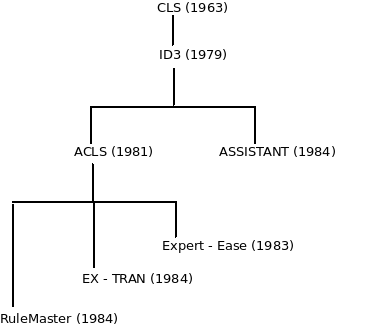
\includegraphics[width=60mm, height=45mm]{Figuras/Arvore/TDIDT.png}\\
	\tiny Fonte: J. R. Quinlan. 
\end{figure} 

Para Quinlan \cite{Quinlan86inductionof}, o pai da família TDIDT é o Sistema de Aprendizagem de Conceito (Concept Learning System – CLS) de Hunt, proposto em 1963, que constrói uma árvore de decisão que visa diminuir o custo de classificar um objeto. Para cada etapa o CLS explora o conjunto de decisões possíveis, seleciona uma ação que minimize o custo, para então mover a um nível abaixo na árvore. O ID3 configura-se, então, como um entre uma série de programas desenvolvidos em função desse Sistema (CLS).

O ACLS \cite{Quinlan86inductionof}, por sua vez, seria uma generalização do ID3. Enquanto que o CLS e o ID3 têm propriedades que possibilitam descrever objetos apenas com valores de um grupo especifico, o ACLS permite propriedades com valores não restritos, podendo ser aplicado para tarefas das mais complexas, tal como o reconhecimento de imagens.

O “Assistant” (ver figura anterior), por sua vez, generaliza atributos do ACLS, permitindo atributos valores contínuos. E, embora não produza uma árvore de decisão iterativa, como acontece com o ID3, tem o poder de escolher um conjunto de treinamento para os objetos disponíveis. Essa classe de algoritmos tem sido bastante utilizada no campo médico, por exemplo.


Ainda na figura anterior, os três sistemas à esquerda são derivações comerciais do ACLS, que não estão relacionados a avanços teóricos consideráveis, mas incorporam inovações simples e de sucesso na geração e utilização de árvores de decisão.

Conforme mencionado, a tarefa das árvores de decisão desse tipo é a de classificação.  Seu produto será, pois, uma classe. Para tal, \cite{Quinlan86inductionof} descreve que a estratégia subjacente a essa árvore é não-incremental, ou seja, um grupo de casos relevantes é apresentado, os exemplos são dados, mas não há uma ordem específica de apresentação dos mesmos. 

Ainda do ponto de vista histórico, no final da década de 80 e início da década de 90 \cite{Kohavi99decisiontree} é desenvolvido o algoritmo C4.5, uma evolução significativa do ID3, que consegue lidar tanto com atributos categóricos, quanto contínuos. É também capaz de lidar com valores desconhecidos, representados por “?” e sendo tratados de forma especial no processo.

No W.E.K.A. (Waikato Environment Knowledge Analysis) é disponibilizada sua implementação, passando a ser chamado J48, que é a implementação na linguagem Java do algoritmo utilizado na pesquisa contemplada nessa dissertação.

O C4.5 é capaz de analisar a medida de ganho, introduzindo um conceito fundamental para o avanço desse algoritmo: a “poda”, que é realizada utilizando medidas estatísticas para identificar e, posteriormente, excluir ramos. Tal processo permite o recorte de ramos que não apresentam contribuição significativa, melhorando o desempenho do algoritmos, que se tornou um dos  mais utilizados na literatura que contempla árvores de decisão. 

São identificadas dois momentos em que são realizadas as podas. O primeiro é o de pré-poda, efetivado no treinamento e que se caracteriza pela interrupção do processo de divisão do nó “em função da avaliação de um conjunto de medidas, transformando o nó em folha rotulada com a classe majoritária” \cite{Simoes2008}. A pós-poda, por sua vez, é executada findo o processo de construção da árvore, e é aplicada recursivamente, na direção de baixo para cima.

Segundo Quinlan \cite{Kohavi99decisiontree}, os dados de entrada do C4.5 são caracterizados por uma coleção de casos de treinamento, cada uma com um tupla de valores para um grupo de atributos (variáveis independentes) e uma classe de atributos (variáveis dependentes). Um atributo, por sua vez, pode ser contínuo ou discreto.

Para Ian e Frank \cite{MachineLearning}, as árvores de decisão geradas a partir do C4.5 podem ser representadas por uma abordagem ``dividir para conquistar'' para resolução de problemas de 
aprendizagem, a partir de um conjunto de instâncias independentes. Os nós em uma árvore de decisão ``testam'' um atributo específico, comparando seu valor com uma constante. No entanto, algumas árvores podem comparar dois atributos com outros ou utilizarem uma função para tal.

O último algoritmo de árvores de decisão que pretendemos contemplar nessa breve revisão histórica é o CART – Classification and Regression Trees \cite{breiman1984}. Esse algoritmo produz tanto árvores de classificação (para o caso de atributos discretos) quanto de regressão (para atributos contínuos). 

O CART é conhecido, sobretudo, pela técnica de partição recursiva binária, tendo em vista que cada nó é dividido em dois outros nós, que podem ser divididos, cada um, em mais dois nós, sucessiva e recursivamente. É estabelecido um conjunto de regras que dão suporte à divisão de cada nó, até a decisão de que a árvore está completa.

Diferentemente do C4.5, o CART não realiza pré-poda. A poda acontece ao final – pós-poda - da árvore gerada, em seu tamanho máximo, e por meio da relação custo-complexidade \cite{breiman1984}, obtendo, muitas vezes, subárvores, que são analisadas e, via de regra, a melhor delas é escolhida.
Ainda no que diz respeito ao CART, o critério de classificação utilizado é o índice de Gini. Esse índice tem como base o cálculo da entropia, e é utilizado frequentemente como parâmetro de pesquisa no campo sócio-econômico.

A entropia é um conceito, utilizado na química e na física, para medir a quantidade de desorganização da matéria. WIENER e SHANON \cite{Pineda2006} lançaram mão desse conceito para analisar a desorganização da informação. Quando há alta entropia, pode-se dizer que a informação está com nível considerável de desorganização ou de medida de incerteza.

No caso das árvores de decisão, a entropia é citada por RUSSEL \& NORVIG \cite{NorvigRussel2004} relacionada ao ganho de informação. Quando um atributo é identificado como aquele que está relacionado a um maior ganho de informação (ou maior redução de entropia), ele é escolhido como o atributo teste para o nó. Tal atributo teria, então, a função de diminuir a aleatoriedade ou impureza nas partições \cite{Simoes2008}. A seguir a equação que representa o cálculo padrão da entropia (já mencionada na seção 2.2.2)
 
\begin{equation}
H_{x}=-\sum_{\forall x \in X}P(x)log_{2}P(x)
\end{equation}

$ H_{x} $ é a medida de entropia, x um atributo do conjunto de variáveis $X$ de variáveis. 

A entropia condicional, formalizada na equação seguinte, é a entropia restante dos atributos de $Y$ no valor $y$ quando o atributo $X$ é dado como $x$ \cite{DecisionTree}:

\begin{equation}
H_{Y|X}= \sum_{x}P(x)H(Y|X=x) =-\sum_{\forall x \in X}P(x) \sum_{\forall y \in Y}P(y|x)log_{2}P(y|x)
\end{equation}

Com essa abordagem é possível reduzir o número de testes necessários para que uma árvore seja produzida.


\subsubsection{Redes Neurais}

%\textbf{Introdução}
\vspace{5mm}

O cérebro humano possui cerca de 10 bilhões de neurônios, que são responsáveis pelo funcionamento do organismo. 
Esses neurônios se conectam entre si, através de sinapses, formando uma Rede Neural capaz de armazenar e processar grande quantidade de informações \cite{NorvigRussel2004}.

De forma semelhante às Redes Neurais naturais, foram desenvolvidas as Redes Neurais Artificiais, que recebem esse nome por se caracterizarem como um sistema cujo funcionamento é semelhante à arquitetura das redes neurais humanas.
 
No início da década de 40, precisamente em 1943, McCulloch e Pitts \cite{Heaton2008} propuseram um modelo simplificado de funcionamento do cérebro humano e, 
a partir dai sugeriram a construção de uma máquina que fosse inspirada nesse funcionamento.


\subsubsection{Definições e aprendizado em Redes Neurais Artificiais}

São várias as definições que podem ser encontradas sobre o que vem a ser uma Rede Neural Artificial (RNA) \cite{Castanheira2008}, em função da complexidade de tal Rede. 
Do ponto de vista computacional, uma RNA configura-se como uma técnica para solucionar problemas de Inteligência Artificial (IA) que estabelece um modelo matemático 
baseado em funções de um modelo neural biológico simplificado, com capacidade de estabelecer concexões sinápticas, bem como, de aprendizado, generalização, associação e abstração.

Os neurônios, nessas redes são conhecidos como Perceptrons. O arranjo em camadas desses perceptrons é chamado \textit{Multilayer Perceptron}, que é responsável pela resolução de problemas mais complexos que não seriam passíveis de resolução pelo modelo 
de neurônio básico. 

São três as camadas usualmente identificadas em uma rede de perceptrons:
\begin{itemize}
 \item Camada de entrada: nessa camada apresenta-se os padrões à rede;
 \item Camadas Intermediárias (ocultas): aqui é realizada a maior parte do processamento por conexões ponderadas. São consideradas como as camadas 
 extratoras de características;
 \item Camada de saída: responsável pela conclusão e apresentação do resultado.
\end{itemize}

As unidades de processamento são conectadas por canais de comunicação, associados a determinado peso, como mostra a Figura 2.17, proposta por McCulloch e Pitts \cite{mcculloch1943logical}.
Esses canais são os  \textit{inputs}, $ I_{1}, I_{2}, I_{3},...,I_{n}$, e cada um tem um peso associado, que serão calibrados de acordo 
com a aproximação do resultado esperado pela rede neural, produzido na saída (fase de ``forward''). Essa aproximação é conhecida como erro ou erro padrão.  Esse erro será propagado de volta à entrada, retroalimentando a rede neural (fase de ``backward''), caso o modelo de rede de aproximação seja o ``backpropagation''. Dessa forma a rede neural se aproxima cada vez mais do resultado que foi previamente estimado na fase de treinamento.

\begin{figure}[htbp!]
\centering
\caption{Perceptron de McCulloch e Pitts}
\vspace{1mm}
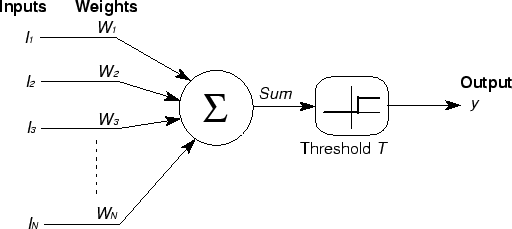
\includegraphics[width=95mm, height=50mm]{Figuras/Neural/Perceptron.png}\\
\tiny Fonte: http://www.din.uem.br/ia/neurais/neural. Acessado em: 01/10/2016
\end{figure}


Uma rede neural passa por um processo aprendizado, resultante de uma fase de treinamento, estabelecido a partir de casos reais, que a faz adquirir, a partir de então, a sistemática que é necessária para executar o processo desejado satisfatoriamente. 
Uma vez ``treinada'' os pesos estão calibrados para solucionar a classe de problemas para o qual foi desenhada. 


O treinamento supervisionado tem sido o mais comumente utilizado em redes neurais \cite{Barreto2002}. 
Em linhas gerais, como o nome indica, no treinamento supervisionado há um agente externo que indica explicitamente à rede um 
comportamento bom ou ruim, com base no padrão de entrada. Os valores iniciais dos pesos são aleatórios, e o ajuste se dá a partir do 
algoritmo de aprendizado, na próxima interação ou ciclo seguinte. São apresentados sinais de entrada e de saída à rede, e os ajustes 
vão sendo feitos paulatinamente. O treinamento pode levar um período considerável de tempo, em função dos ajustes que vão sendo 
realizados. O treinamento é concluído quando a rede neural atinge um determinado patamar de desempenho, tendo alcançado a precisão 
estatística esperada. 
Não havendo mais necessidade de treinamento, “congela-se” os pesos, para sua aplicação. 

O aprendizado não supervisionado, por sua vez, não depende de um agente externo, pois funciona de forma autorregulatória, apresentando 
mecanismos que analisam as regularidades ou tendências dos padrões de entrada, possuindo a capacidade de se adaptar automaticamente às 
necessidades da rede. 

%\pagebreak

\section{Métricas aplicadas à mineração}

Quando são desenvolvidos sistemas de predição e análise de diagnóstico, avalia-se o desempenho e a qualidade dos resultados encontrados.
Um método gráfico eficiente para detecção e avaliação da qualidade de sinais, conhecido como \textit{Receiver Operating Characteristic} -- ROC, ou curva ROC \cite{ROC},
foi criado e desenvolvido na década de 50 do século passado, para avaliar a qualidade da transmissão de sinais em um canal com ruído.
Recentemente a curva ROC tem sido adotada em Mineração de dados e Aprendizagem de Máquina \cite{MD_AM}, em sistemas de suporte à decisão na medicina, para analisar a qualidade da detecção 
de um determinado teste bioquímico, na psicologia para detecção de estímulos \cite{Discriminativo} em pacientes, e na radiologia para classificação de imagens.

Essas métricas são amplamente utilizadas na classificação binária de resultados contínuos. Para isso ser construído utiliza-se a Matriz de Contingência que classifica as probabilidades como:
verdadeiro positivo, falso positivo, falso negativo e verdadeiro negativo, respectivamente \textit{True Positive -- TP, False Positive -- FP, False Negative -- FN e True Negative -- TN },
também conhecida como matriz de confusão, descrita na tabela a seguir:

%tabela 5
\begin{table}[ht]
\centering
\caption{Matriz de Confusão}
\vspace{1mm}
\begin{tabular}{l|c|c}
\hline
\textbf{} & \textbf{Predito} & \textbf{}\\
\hline
\textbf{Real}  & TP   FN & Positive -- POS\\
\textbf{Real}  & FP   TN & Negative -- NEG\\
\hline
   ---         & PP   PN &    ---         \\
\end{tabular}
\\
\tiny Fonte: \cite{Bradley1997}
\end{table}

A matriz da Tabela 2.3 sintetiza a matriz da Tabela 2.4, portanto as duas tabelas são equivalentes.

%tabela 6
\begin{table}[ht]
\centering
\caption{Matriz modelo de Confusão}
\vspace{1mm}
\begin{tabular}{l|c|c}
\hline
\textbf{}           & \textbf{Y}     \textbf{$\bar{Y}$}   & \textbf{}\\
\hline
\textbf{X}          & P(X,Y)         P(X,$\bar{Y}$)       & Positive -- POS\\
\textbf{$\bar{X}$}  & P($\bar{X}$,Y) P($\bar{X},\bar{Y}$) & Negative -- NEG\\
\hline
   ---              & P(Y)           P($\bar{Y}$)         &     ---        \\
\end{tabular}
\\
\tiny Fonte: \cite{Bradley1997}
\end{table}


De acordo com as probabilidades condicionais temos:

\begin{equation}
 P(X,Y) = P(X|Y).P(Y) = P(Y|X).P(X)
\end{equation}

Então, a taxa de verdadeiros positivos será $P(Y|X)$ e a probabilidade de falsos alarmes ou taxa de falsos positivos será $P(Y,\bar{Y})$, a barra sobrescrita em $\bar{X}$
(ou $\bar{Y}$) representa negação. \\
A curva ROC será construída cruzando-se a taxa dos verdadeiros positivos (tpr = P(Y|X)) com a taxa dos falsos positivos (fpr = P(Y,$\bar{X}$)).


\pagebreak

\subsection{Classificação para análise preditiva}

Classificação é um processo para encontrar um modelo que descreve e distingue classes de dados. 
Esse modelo tem como base de análise um conjunto de treinamento (i.e. objetos de dados para os quais 
serão encontrados rótulos que os classifiquem). 

Esse modelo é usado para predizer quais rótulos de classes terão os objetos desconhecidos.
O modelo pode ser representado por regras de classificação do tipo ``IF - THEN'', por árvores de decisão, redes neurais e outros. 
Regras de classificação se distinguem de regras de indução da seguinte forma:
\begin{itemize}
	\item Uma regra de classificação poderia ser: $if$ L $then$ class = $C_{1}$ ou $if$ L $then$  $C_{1}$
	\item Uma regra de indução seria: $ if$ L $then$ R que por sua vez produz novas regras 
\end{itemize}

%\singlespace
%\vspace{2cm}

\begin{figure}[ht] \unitlength= 1mm \thicklines
	\centering{
		\begin{picture}(100,6)
		\put(0,0){\framebox(115,6)} \put(3,2){$age(X,``youth")$ AND $income(X,``high")  \to classe (X,``A")$}
		\put(0,-7){\framebox(113,6)} \put(3,-5){$age(X,``youth")$ AND $income(X,``low") \to classe (X,``B")$}
		\put(0,-14){\framebox(85,6)} \put(3,-12){$age(X,``middle-aged")$  $\to classe (X,``B")$}
		\put(0,-21){\framebox(70,6)} \put(3,-19){$age(X,``senior")$  $ \to classe (X,``B")$}
		\end{picture}
	}
\end{figure}

\vspace{3cm} 

A Figura 2.18 representa uma rede neural com as mesmas características da árvore de decisão anterior:
\begin{figure}[!ht]
	\centering
	\caption{Rede Neural}
	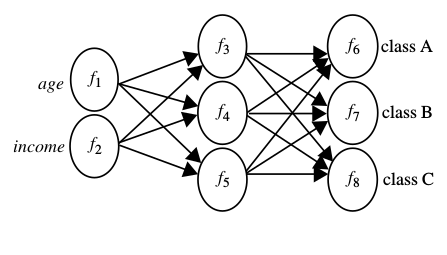
\includegraphics[width=85mm, height=38mm]{Figuras/BigData/redeneural.png}\\
	\tiny Fonte: Han, J. and Kamber, M. 
\end{figure}  

As árvores de decisão produzem regras de indução, são algoritmos rápidos, contudo dados impuros podem comprometer o desempenho desse algoritmo. 
A fase de extração dos dados do é fortemente influenciáveis pelas variáveis escolhidas, \cite{DecisionTree} 
isso pode representar o desafio maior para implementar esta técnica. 

Outro problema que pode ser encontrado em algoritmos de aprendizagem é o ``overfitting'' ou superadaptação aos modelos.
Segundo RUSSEL E NORVIG \cite{NorvigRussel2004}  \footnote{Foi observado que redes neurais muito grandes \textit{generalizam} bem, 
\textit{desde que os pesos sejam mantidos pequenos}. Essa restrição mantém os valores de ativação na região 
\textit{linear} da função sigmóide g(x) onde x é próximo de zero. Por sua vez isso faz com que a rede se comporte 
como uma função linear, com um número muito menor de parâmetros.} o ``overfitting'' ocorre quando o número atributos é grande.


\subsection{Pesquisas envolvendo inteligência artificial e tráfego em rodovias}

Nesta sessão apresentaremos algumas pesquisas realizadas no Brasil e em outras partes do mundo, que contemplam elementos de interesse para nossa pesquisa: tráfego em rodovias e o uso de técnicas de inteligência artificial, como árvores de decisão e redes neurais, dentre outras.

Para tal, tomamos como referência a última década de produção, priorizando artigos a partir de 2010, embora tenham sido identificadas pesquisas desde meados dos anos 90, já contemplando tráfego urbano ou em rodovias e inteligência artificial.

No Brasil, sobretudo no eixo sul-sudeste, algumas pesquisas têm sido conduzidas nesse campo. Corrêa \cite{correa2008aplicaccao} desenvolveu um estudo exploratório, em que buscou identificar pesquisas no Brasil que tratassem da utilização de redes neurais aplicadas ao setor de transporte, comparando com aquelas produzidas sob a mesma temática, em países desenvolvidos. Essa autora identifica a produção de pesquisas nesse cenário desde os anos 90, corroborando a análise que fizemos sobre pesquisas que foram produzidas nesse campo, com auxílio da ferramenta de busca google acadêmico.

Identificamos campos de interesse que podemos resumir da seguinte forma: pesquisas interessadas em utilizar técnicas de IA para identificar comportamento de tráfego ou causas de acidentes graves, notadamente os acidentes fatais, podendo, ou não preocupar-se com a predição de acidentes futuros, mas sem propor algum tipo de solução prática ou desenvolvimento de ferramentas auxiliares do tráfego. Outro campo de interesse foi pela utilização da IA para proposição de soluções práticas, aplicativos, ferramentas, para lidar com os constrangimentos de tráfego, sem preocupação específica com, por exemplo, causas de acidentes fatais. Finalmente outro campo de interesse mobiliza técnicas de IA e que além da identificação de problemas relativos ao tráfego em vias urbanas e rodovias, preocupa-se com a modelização e predição de rotas alternativas, nas quais essa pesquisa se insere, embora seja importante destacar que há aspectos dos outros dois grupos que também nos interessam, como, por exemplo, as causas de acidentes, sobretudo que culminam com óbitos em acidentes rodoviários. 

A seguir, destacamos alguns estudos, que mesmo oriundos de contextos tão diversos, apontam para interesses semelhantes. Optamos por destacar pesquisas relacionadas às mais diversas regiões, no sentido de destacar o quanto esse campo é vasto e de interesse mundial.

Em uma pesquisa conduzida nos Estados Unidos, com dados obtidos a partir do do Sistema de Relatório de Análise de Fatalidades (FARS), no Alabama, Shanthi e Ramani \cite{shanthi2012feature} buscou analisar em que medida os algoritmos de classificação de mineração de dados são eficazes para previsão dos fatores que influenciam acidentes de trânsito, levando em conta a gravidade da lesão decorrente do acidente. Nessa pesquisa foi comparado o desempenho de algoritmos como C4.5, CR-T, ID3, CS-CRT, CS-MC4, Naïve Bayes e Árvore de randomização, para modelar a gravidade da lesão ocorrida no acidente. A acurácia foi avaliada com base na precisão e valores de recall e os resultados apontaram para a eficácia desses algoritmos, com destaque para as árvores de randomização.

Boa parte das pesquisas desenvolvidas no Brasil têm focado na identificação de problemas relacionados ao congestionamento de vias urbanas ou rodovias no interior do estado, propondo, a partir da utilização de técnicas de IA, como redes neurais, árvores de decisão, lógica fuzzy, identificar o comportamento dos veículos nas vias, um exemplo é a pesquisa de Ferreira \cite{ferreira2011combinaccao}, que buscou utilizar combinação de técnicas de IA para previsão do comportamento do tráfego na cidade de São Paulo.

Pertencente a outro campo de interesse - aquele voltado para a proposição de soluções práticas - Braga et al \cite{braga2014planejamento} utilizaram o algoritmo de IA Anytime e executaram os testes na Plataforma Raspberry, com o objetivo de estabelecer um planejamento de rotas nas malhas viárias das cidades de Manaus e do Rio de Janeiro. A plataforma utilizada na pesquisa mostrou-se eficaz para a proposição de um protótipo de planejamento de rota, para uso veicular e abre caminho para o desenvolvimento de um aplicativo para smartphones.  

Outra pesquisa, conduzida em Portugal \cite{dos2016previsao}, propôs o desenvolvimento de soluções inteligentes, a partir do uso de data mining e técnicas de simulação, para estabelecer predições das condições de tráfego em tempo real, de modo a conter o aumento dos congestionamentos em rodovias e região metropolitana. Essa recente pesquisa aproxima-se, em certo sentido, do nosso interesse, uma vez que tem como foco uma abordagem de predição, tal qual propomos nesta pesquisa. No caso da pesquisa desenvolvida por Reis, os dados históricos utilizados foram capturados a partir dos sensores localizados nas estradas, diferentemente de nossa proposta, que contempla dados históricos da Polícia Rodoviária Federal de Pernambuco (mineração de dados) e da rede social Twitter (mineração em textos).

A preocupação com acidentes graves, muitos deles implicando em mortes, também tem destaque em pesquisas nos países desenvolvidos ou onde é sabido haver problemas ligados ao tráfego nas capitais e nas importantes cidades do interior, como é o caso de alguns países do Oriente Médio. Essas pesquisas estão relacioandas ao primeiro campo que destacamos acima: as que buscam identificar e alertar as autoridades sobre o impacto de acidentes fatais relacionados ao tráfego.

Uma pesquisa conduzida nos Estados Unidos por Chong, Abraham, Paprzycki \cite{chong2004traffic}, destaca o grande impacto social que esse tipo de fatalidade promove. Esses pequisadores utilizaram as redes neurais e árvores de decisão para modelar os acidentes graves e fatais, identificando três causas fundamentais que promovem acidentes dessa natureza: a não utilização de cinto de segurança, a condição de luminosidade na rodovia (que em nossa pesquisa está incluída na variável condições de visibilidade) e consumo de álcool pelo condutor.

Pesquisa semelhante foi desenvolvida por Akgüngör e Dogan \cite{akgungor2009artificial}, que utilizaram redes neurais e algoritmos genéticos para apropor um modelo para estimar o número de acidentes (A), com vítimas fatais (F) e prejuízos (I), em Ankara (Turquia), utilizando dados de um espaço temporal de 20 anos (1986 a 2006), de modo a oferecer um retrato fiel dos impactos sociais causados pelas condições precárias do tráfego nas grandes cidades turcas.

Kashani, Shariat-Mohaymany, Ranjbari \cite{tavakoli2011data}, em pesquisa desenvolvida no Irã, utilizaram a árvore de regressão e classificação (CART) para analisar os acidentes fatais de trânsito que acontecem no Irã. Segundo os dados dessa pesquisa, setenta por cento dos acidentes com vítimas fatais no Irã acontecem nas áreas rurais. A pesquisa identificou que as principais causas de morte relacionadas ao tráfego são: a ausência do uso de cinto de segurança, as ultrapassagens indevidas e o consume de álcool por parte do condutor. Tomando como referência a nossa pesquisa, destacamos que as causas consideradas como mais relevantes dizem respeito ao condutor do veículo, mais do que às condições da via.

Em uma pesquisa conduzida na Jordânia, Jadaan, Al-Fayyad e Gammoh \cite{jadaan2014prediction}, tiveram como objetivo propor um modelo de predição de futuros acidentes de tráfego, utilizando-se de Redes Neurais. A pesquisa considerou o espaço temporal entre 1990 e 2011, e tomou como dados de entrada das Redes Neurais: número de veículos registrados, população, comprimento de estradas pavimentadas, produto interno bruto. Foram propostos quarto modelos alternativos, e um deles (4o.) mostrou-se o mais adequado, com coeficiente de determinação (R2 =0.992), a partir do qual propuseram o modelo de predição, considerando os dados atuais e o número previsto de acidentes.

Beshah e Hill \cite{beshah2010mining} desenvolveram uma pesquisa na Etiópia, utlizando algoritmos de IA, para identificar as principais causas de acidentes graves, principalmente aqueles com mortes, que vitimizam aproximadamente 1 milhão e 200 mil pessoas, além de deixar cerca de 50 milhões de feridos. Os pesquisadores utilizaram árvores de decisão, Naïve Bayes e outros classificadores, para identificar as principais causas dos acidentes. Consideraram algumas variáveis que também interessaram particularmente à nossa pesquisa, como condições de visibilidade da via, sentido da via, gravidade do acidente. Também conforme o interesse de nossa pesquisa, o estudo em questão interessou-se pelo estabelecimento de um modelo preditivo, a partir das tecnologias de IA utilizadas.

Interessados pela mesma temática, Olutayo e Eludire \cite{olutayo2014traffic} desenvolveram pesquisa na Nigéria, utilizando técnicas de Árvores de Decisão e Redes Neurais para analisar o tráfego em rodovias de tráfego intenso, com o objetivo de, segundo eles, reduzir a carnificina nas grandes rodovias do país. Coletaram dados históricos da instituição de segurança rodoviária daquele país, referentes a 40 km de rodovia, entre as cidades de Ibadan e Lagos, classificando-os como contínuos ou como categóricos. Para os dados contínuos foram utilizadas a técnica de Redes Neurais Artificiais, e os dados categóricos foram tratados com Árvores de Decisão. Os resultados apontaram que as principais causas de acidentes fatais são rupture de pneu, perda de controle e alta velocidade. Assim como outros estudos, as causas relacionadas aos condutores aparecem como aquelas mais fortemente associadas a acidentes fatais. Os autores propuseram, ainda, estabelecer uma comparação entre RNA e AD, como técnicas de IA associadas à resolução do problema de pesquisa, e identificaram que as RNA um relatório de erro mais baixo, bem como maior número de instâncias corretamente classificadas e taxa de precisão mais elevada.

Também com o objetivo de comparar os resultado obtidos utilizando Redes Neurais e Árvores de Decisão, pesquisa conduzida na Tailândia \cite{thianniwet2010classification} propôs uma técnica para identificar níveis de congestionamento em rodovias, com base nos dados de sensores de velocidade de alta acurácia; e utilizaram GPS, webcam e uma pesquisa de opinião, essa última para detector percepções humanas/dos condutores sobre os níveis de congestionamento. Essa pesquisa identificou o J48 como o algoritmo de aprendizagem que mostrou o melhor resultado, com acurácia de 91,29\%. Um aspecto que diferenciou essa pesquisa das demais, foi o fato de que considerou as percepções humanas para sua análise. Em nossa pesquisa, os dados obtidos a partir do Twitter e a mineração de textos e análise sentimental, permitiu-nos, igualmente, contemplar a dimensão humana, para além da utilização de dados históricos.

Outros estudos poderiam ainda ser considerados, contemplando ainda a comparação entre algoritmos para gestão segurança rodoviária no sul da Itália \cite{de2015comparison} análise de acidentes em áreas rurais da Espanha \cite{de2011analysis};  utilização da Plataforma GIS para o desenvolvimento de um sistema de reconhecimento automático de acidentes de trânsito na rodovia Konya-Afyonkarahisar, na Turquia \cite{durduran2010decision}, mas acreditamos ter feito o levantamento dos principais pesquisas desenvolvidas nesse campo, na atualidade, o que corrobora com o que discutimos sobre a importância de desenvolvermos um estudo dessa naturea, sobretudo contemplando aspectoas ainda não encontrados na literature, como a integração das redes socias a essas pesquisas, propondo um trabalho de mineração de texto e análise sentimental, em articulação com os dados produzidos pelos algoritmos de IA.

\pagebreak

A Tabela 2.5 demonstra que pesquisas relacionadas com acidentes rodoviários é um fenômeno mundial e uma preocupação dos governos, pelo grande número de sinistros com  óbitos.

%tabela 5
\begin{table}[!ht]
	\centering
	\caption{Tabela resumo das pesquisas em acidentes pelo mundo}
	\vspace{1mm}
	\begin{tabular}{l|c|c|c}
		\hline
		\textbf{Ano} & \textbf{País} & \textbf{Tecnica IA} & \textbf{Aplicação}\\
		\hline
		2000 & Brasil & RNA & Transportes\\
		2002 & Brasil & Anytime  & Planejamento de Rotas\\
		2004 & EUA & AD e RNA & Acidentes de Trânsito \\
		2008 & EUA & C4.5, CS-CRT, NB e AD & Acidentes de Trânsito\\
		2009 & Brasil & RNA, AD, FL  & Congestionamento no Trânsito\\
		2010 & Etiópia & AD, NB, KNN & Acidentes de Trânsito \\	
		2010 & Tailândia & AD e RNA & Congestionamento no Trânsito \\	
		2011 & Turquia & RNA e AG & Acidentes de Trânsito \\
		2011 & Irã & CART & Acidentes de Trânsito \\
		2011 & Espanha & RB & Acidentes em estradas Rurais \\		
		2014 & Jordânia & RNA & Acidentes de Trânsito \\
		2014 & Nigéria & RNA e AD & Acidentes de Trânsito \\		
		2015 & Itália & RNA e AD & Gestão de Segurança no Trânsito \\		
		2016 & Portugal & Q-Learning, SARSA, KNN, AD & Congestionamento no Trânsito\\
		
	\end{tabular}
\end{table}

Países em vias de desenvolvimento, com infraestrutura deficitária, condutores mal disciplinados formam o maior contingente das pesquisas e parecem ser os principais causadores de grande número de sinistro nas rodovias.

As técnicas mais utilizadas nos 14 artigos relacionados foram: Árvores de Decisão (AD) em 8, Redes Neurais Artificiais (RNA) em 7, Naïve Bayrs em 3 e KNN em 2 artigos. 
Um detalhe que despertou nosso interesse é que Redes Neurais e Árvores de Decisão foram utilizadas conjuntamente em 5 dos artigos distintos, dentre outras técnicas.
Essa preferência foi levada em consideração e guiu-nos, a priori, pelos caminhos da nossa pesquisa.